
% Szkielet dla pracy inżynierskiej pisanej w języku polskim.

\documentclass[polish,bachelor,a4paper,oneside]{ppfcmthesis}

\usepackage[utf8]{inputenc}
\usepackage[T1]{fontenc}
\usepackage{usecase}
\usepackage{float}
\usepackage[table]{xcolor}
\usepackage{mat}
\usepackage{verbatim}
\usepackage{pdflscape}
\usepackage{longtable}

\hyphenation{roz-sze-rza-ją-cych}

% Authors of the thesis here. Separate them with \and
\author{%
   Krzysztof Marian Borowiak \album{94269} \and 
   Maciej Trojan \album{94378} \and 
   Krzysztof Urbaniak \album{94381} \and 
   Łukasz Wieczorek \album{94385}}
\title{iQuest -- system rozszerzonych ankiet~studenckich}                   % Note how we protect the final title phrase from breaking
\ppsupervisor{dr hab.~inż.~Bartosz Walter} % Your supervisor comes here.
\ppyear{2013}                                         % Year of final submission (not graduation!)


\begin{document}

% Front matter starts here
\frontmatter\pagestyle{empty}%
\maketitle\cleardoublepage%

% Blank info page for "karta dyplomowa"
\thispagestyle{empty}\vspace*{\fill}%
\begin{center}Tutaj przychodzi karta pracy dyplomowej;\\oryginał wstawiamy do wersji dla archiwum PP, w pozostałych kopiach wstawiamy ksero.\end{center}%
\vfill\cleardoublepage%

% Table of contents.
\pagenumbering{Roman}\pagestyle{ppfcmthesis}%
\tableofcontents* \cleardoublepage%

% Main content of your thesis starts here.
\mainmatter%
\chapter{Wprowadzenie}
\label{Chapter1}

\section{Opis problemu i koncepcja jego rozwiązania}
\label{Chapter11}

\subsection{Problem}
\label{Chapter111}

Podstawą każdej działalności jest warunkująca ją potrzeba. Niemożliwą jest jednak analiza potrzeb, bez wcześniejszego ich zbadania. Najłatwiejszą i najbardziej rozpowszechnioną metodą pozyskiwania wiedzy na jakiś temat jest pytanie o to osób związanych ze sprawą. Kiedy pytań jest wiele, a liczba potencjalnych respondentów osiąga poziom kilkudziesięciu tysięcy osób, zadawanie pytań wymaga usystematyzowania. Podobnie wygląda kwestia metodyki ich dostarczania do odpowiadających oraz gromadzenia odpowiedzi. Rozwiązaniem tego zagadnienia jest równie proste, co skuteczne narzędzie badań, pozwalające na gromadzenie danych - ankieta. \\

Ankieta pozwala na nieinwazyjne, anonimowe i masowe pozyskiwanie opinii respondentów na zadany temat, a dzięki zastosowaniu różnych metod statystycznych, także na ocenę zdania całej populacji. W kontekście każdej jednostki, zrzeszającej większą grupę osób, jak zakład pracy, czy jednostka szkolnictwa wyższego, jaką jest Politechnika Poznańska, ankietowanie jest niezwykle potrzebne, celem zapewnienia prawidłowej pracy. Bez informacji zwrotnej (ang.~\definicja{feedback}) praktycznie nie ma możliwości precyzyjnej analizy poprawności podejmowanych działań, co w efekcie zawsze będzie prowadzić do spiętrzającej się fali problemów. Za przykład może posłużyć sytuacja, gdy nie posiadając wiedzy o nieodpowiednim (zdaniem studentów i prowadzących zajęcia) wyposażeniu sali laboratoryjnej, władze uczelni ustalają harmonogram zajęć, zwiększający obciążenie tego pomieszczenia. Efektem takiego działania byłby spadek jakości kształcenia studentów korzystających z tego laboratorium. \\

W ostatnich latach\footnote{Mowa o okresie 2008-2013, który jest znany autorom niniejszej Pracy Dyplomowej.} Politechnika Poznańska posiadała szerokie spektrum narzędzi do pozyskiwania wiedzy o swoim działaniu i oferowanych usługach, funkcjonujących w zgodzie ze Statutem Politechniki Poznańskiej\footnote{Zapis odnośnie dokonywania oceny nauczyciela akademickiego z uwzględnieniem oceny studentów\cite{AP:SPP11}.}. Niestety, gros z nich wzajemnie się wykluczał. Przykładowy student na Wydziale Informatyki\footnote{Do 2010 roku -- Wydziale Informatyki i Zarządzania} poddawany był ankietom: elektronicznym na poziomie Uczelni, jak i Wydziału, ,,papierowym'' na poziomie Uczelni oraz Samorządu Studentów, a ponadto dodatkowej ankietyzacji w ramach niektórych zajęć dydaktycznych. \\

Żaden spośród tych ,,systemów'' ankietyzacji nie posiadał odpowiednich zabezpieczeń, wymaganych do zapewnienia wymierności ich wyników (jak np.~zagwarantowanie, aby nikt nie wziął w ankiecie udziału więcej niż jeden raz, czy uniemożliwienie wypełnienia ankiety przeznaczonej dla innego wydziału, kierunku). Brak wymiernych efektów udziału w tych badaniach, podobnie jak ich mnogość i dezorientacja zwiżana z pytaniem ,,kto tak naprawdę pozyskuje informacje'', działały tu na niekorzyść ankietujących. Ważnym jest też fakt, że istniała tylko jedna, globalna grupa docelowa -- studenci Politechniki Poznańskiej. \\

Ustawa o Szkolnictwie Wyższym wymaga od uczelni wyższych badania nie tylko aktualnej społeczności studenckiej, lecz także jej absolwentów\cite{AP:PoSW05}. Sprawdzane powinny być takie czynniki, jak rozwój karier czy satysfakcja z zapewnianych usług. Niestety, na Politechnice Poznańskiej brak jest odpowiednich narzędzi do prowadzenia tego rodzaju analiz. Nawiązując więc do wcześniejszych twierdzeń, potencjalna katastrofa (jak niezauważony spadek jakości usług, prowadzący do zmniejszenia satysfakcji odbiorców ze względu na brak podjęcia odpowiednich działań i w efekcie spadku prestiżu Uczelni) to jedynie kwestia czasu. \\

\subsection{Proponowane rozwiązanie}
\label{Chapter112}

Najłatwiejszym i -- w opinii autorów niniejszego dokumentu -- najlepiej popartym logicznymi argumentami rozwiązaniem, jest stworzenie jednego, jednolitego, globalnego i prostego w obsłudze systemu prowadzenia badań i ankiet dla różnych grup docelowych, obejmujących wszystkich aktualnych i byłych studentów Politechniki Poznańskiej. Aby zapewnić dostępność oraz prostotę wdrożenia systemu, który na to pozwoli, zostanie on wykonany za pomocą technologii internetowych, co umożliwi też jego obsługę z użyciem dowolnej popularnej przeglądarki internetowej dostępnej na rynku. \\

W trakcie analizy problemu ustalono, że koniecznym będzie także zapewnienie swojego rodzaju ,,zachęty'' dla potencjalnych respondentów -- o ile bowiem studentowi może zależeć na rozwoju jego uczelni, o tyle absolwent nie będzie czerpał z tego tytułu żadnych wymiernych korzyści. Wybrane dla systemu iQuest rozwiązanie obejmuje więc też element zachęcający do korzystania z systemu, jakim jest udzielanie im dostępu do unikalnych materiałów dydaktyczno-naukowych. \\

Aby zapewnić, że pozyskane w badaniach dane są prawidłowe, w proponowanym rozwiązaniu znajdą się systemy autoryzacji osób ankietowanych. Jest to jednak jedyny element wymagający sprawdzenia tożsamości respondenta -- same wyniki będą dla ankietera całkowicie anonimowe. \\

\section{Ograniczenia i zagrożenia dla projektu}
\label{Chapter12}

Największym ograniczeniem, a zarazem zagrożeniem dla całego projektu jest kwestia zachęty studentów i absolwentów do korzystania z nowego systemu ankietowania. Popularność całego systemu zależy w głównej mierze właśnie od tego, jakie materiały będą za jego pośrednictwem udostępniane oraz jakie będą warunki uzyskania dostępu do nich. \\

Rozpatrując jednak tę kwestię ze strony implementacyjnej, sporym zagrożeniem okazuje się wymaganie stosowania rozwiązań ,,otwartych'' i ,,wolnych'', ograniczające spektrum możliwych do wykorzystania technologii i zasobów. W tej kategorii, za poważne ograniczenie należałoby także uznać wyznaczony z góry termin zakończenia prac. Na projektowanie, implementację i wdrożenie rozwiązania przewidziany jest jedynie okres od września 2012, do lutego 2013. Uzupełniając tę kwestię o fakt braku wcześniejszego doświadczenia zespołu przy realizacji projektów opartych na technologiach internetowych, spełnienie wszystkich wymagań związanych z projektem może okazać się utrudnione. \\

Ostatecznie jednak, kwestia zachęty dla respondentów -- choć istotna dla powodzenia systemu w przyszłości -- w fazie tworzenia może być potraktowana jako poboczna. Kwestię ograniczonego czasu można natomiast nadrobić, stosując odpowiednie metody zarządzania czasem. Największym zagrożeniem pozostaje więc brak wcześniejszego doświadczenia w tego typu projektach oraz ograniczenia dotyczące możliwych do zastosowania technologii. \\

\section{Cele projektu}
\label{Chapter13}

Celem projektu \textit{iQuest} jest zbudowanie systemu umożliwiającego łatwe przeprowadzanie ankiet wśród studentów i absolwentów uczelni. System ten powinien:
\begin{itemize}
\item{zapewnić spełnienie przez Uczelnię zapisów Ustawy ,,Prawo o Szkolnictwie Wyższym'' dotyczących monitorowania rozwoju absolwentów Uczelni\cite{AP:PoSW05}}
\item{ujednolicić uczelniany system pozyskiwania informacji}
\item{oferować dużą elastyczność:
\begin{itemize}
\item{przy definiowaniu różnorodnych ankiet}
\item{przy tworzeniu i hierarchizacji grup respondentów}
\item{przy zachęcaniu do uczestnictwa w niej przez potencjalnych Respondentów}
\end{itemize}}
\item{oferować rozbudowane możliwości raportowania}
\item{odciążyć pracowników uczelni oraz Samorząd Studentów z obowiązków związanych z przeprowadzaniem konwencjonalnych (,,papierowych'') ankiet}
\end{itemize}

\section{Omówienie pracy}
\label{Chapter14}

{\color{red}Do uzupełnienia po ukończeniu reszty pracy}

%Tutaj piszemy o celu samego dokumentu oraz ewentualnych konwencjach, jakie przyjęliśmy podczas opisywania różnych rzeczy. Dla systemu BIS-2 ten fragment wyglądał tak:
%
%\textit{Niniejszy dokument opisuje system System informacji bibliometrycznej (ang.~\definicja{Bibliometric Information System}) zwanego dalej BIS-2 (dla odróżnienia od wersji pilotażowej), który realizuje koncepcję przytoczoną w~punkcie \ref{Chapter11}. Praca ma formę dokumentacji technicznej dla osób, które zamierzają wdrażać i~obsługiwać system, ale także opisuje ideę stojącą za implementacją poszczególnych części projektu z~odniesieniami do literatury. Ponadto, jest to również praca dyplomowa inżynierska, zatem jej odbiorcami są także członkowie komisji egzaminacyjnej.}
%
%Następnie musicie napisać, co zawierają poszczególne rozdziały. U nas wyglądało to tak:
%
%\textit{W rozdziale \ref{Chapter2}. rozszerzono koncepcję projektu o~przedstawienie aktorów oraz obiektów biznesowych, a~także przybliżono scenariusze operacyjne w~postaci przypadków użycia. Specyfikację wymagań oprogramowania przedstawiono w rozdziałach \ref{Chapter3}.~(funkcjonalne) oraz w~\ref{Chapter4}.~(pozafunkcjonalne). W~rozdziale \ref{Chapter5}.~omówiono architekturę systemu na wyższym poziomie abstrakcji. Uzasadnienie wyboru technologii, opis implementacji i~koncepcji znajduje się w~rozdziale \ref{Chapter6}. Informacje dotyczące zapewniania jakości zostały opisane w~rozdziale \ref{Chapter7}. W~rozdziale \ref{Chapter8}.~umieszczono opis zarządzania wersjami i~sposobu pracy nad projektem. Zebrane wnioski i~doświadczenia zawarto w~rozdziale \ref{Chapter9}. W~dodatkach opisano wkład poszczególnych osób i~informacje uzupełniające. Ostatnią część dokumentu stanowi wykaz literatury przybliżający zagadnienia opisane w~pracy.}

%%%%%%%%%%%%%%%%%%%%%%%%%%%%%%%%%%%%%%%%%%%%%%%%

%Oto przykład tekstu, do którego istnieje adnotacja na dole strony\footnote{To jest właśnie odnośnik.}. Do bibliografii odnosimy się w taki sposób \cite{Hirsch:HIR05}. Dla oznaczenia wszelkich terminów używany znacznika ,,definicja'': \definicja{Termin z definicji}. Natomiast, jeśli chcemy odnieść się do innego miejsca w dokumencie (które jest oznaczone pewną etykietą): \ref{Chapter12}. Łamanie strony odbywa się poprzez znacznik ,,pagebreak''. Po skrótach z kropką warto używać tyldy (np.~tak). Link podajemy poprzez znacznik ,,url'' (\url{www.google.pl}).

%Do takiego ,,zwykłego'' myślnika używamy podwójnego znaku ,,-'', a pojedynczego do łączenia bezpośrednio dwóch wyrażeń. Potrójny stosujemy, jak chcemy gdzieś pokazać brak informacji.

%Kompilację tego dokumentu najwygodniej zacząć od zainstalowania MikTeXa oraz przygotowana pliku render.bat, którego treść przedstawia się następująco:

%\begin{verbatim}
%@echo off
%
%pdflatex thesis-bachelor-polski.tex 
%bibtex   thesis-bachelor-polski
%pdflatex thesis-bachelor-polski.tex 
%pdflatex thesis-bachelor-polski.tex 
%
%del *.aux *.bak *.log *.blg *.bbl *.toc *.out
%\end{verbatim}
%
%Potrójna kompilacja to nie wymysł szalonego programisty, który uważa, że ,,wtedy lepiej się skompiluje'', ale rzeczywista potrzeba wynikająca z poprawnego powiązania ze sobą wszystkich odwołań w dokumencie. Po uruchomieniu takiego pliku .bat (jeśli wszystko pójdzie dobrze), powinien się utworzyć plik .pdf. Nie poleca się uruchamiania skryptu, gdy mamy otwartą aktualną wersję pliku .pdf. Przy pierwszym uruchomieniu, MikTeX prawdopodobnie będzie prosił o pozwolenie na pobranie wymaganych pakietów. UWAGA! Podczas kompilacji być może trzeba będzie trzy razy potwierdzać zaistnienie jakiegoś błędu związanego ze znacznikiem ,,ppcolophon'' -- jak potwierdzicie to Enterem, to kompilacja pójdzie dalej i wszystko skończy się szczęśliwie. To wynika z jakiejś konstrukcji w szablonie udostępnianym przez uczelnię.
%
%W tym podrozdziale generalnie znajduje się opis problemu, jaki doprowadził do powstania koncepcji Waszego systemu. Umieszcza się tu także ogólny opis tego, co Wasz system powinien robić, jakie ma zastosowanie (fachowo to się nazywa ,,problem i jego implikacje (znaczenie)'' oraz ,,cel biznesowy''). 
%

%%%%%%%%%%%%%%%%%%%%%%%%%%%%%%%%%%%%%%%%%%%%%%%%%%%%%%%%%%

%\section{Omówienie pracy}
%\label{Chapter12}
%
%Tutaj piszemy o celu samego dokumentu oraz ewentualnych konwencjach, jakie przyjęliśmy podczas opisywania różnych rzeczy. Dla systemu BIS-2 ten fragment wyglądał tak:
%
%\textit{Niniejszy dokument opisuje system System informacji bibliometrycznej (ang.~\definicja{Bibliometric Information System}) zwanego dalej BIS-2 (dla odróżnienia od wersji pilotażowej), który realizuje koncepcję przytoczoną w~punkcie \ref{Chapter11}. Praca ma formę dokumentacji technicznej dla osób, które zamierzają wdrażać i~obsługiwać system, ale także opisuje ideę stojącą za implementacją poszczególnych części projektu z~odniesieniami do literatury. Ponadto, jest to również praca dyplomowa inżynierska, zatem jej odbiorcami są także członkowie komisji egzaminacyjnej.}
%
%Następnie musicie napisać, co zawierają poszczególne rozdziały. U nas wyglądało to tak:
%
%\textit{W rozdziale \ref{Chapter2}. rozszerzono koncepcję projektu o~przedstawienie aktorów oraz obiektów biznesowych, a~także przybliżono scenariusze operacyjne w~postaci przypadków użycia. Specyfikację wymagań oprogramowania przedstawiono w rozdziałach \ref{Chapter3}.~(funkcjonalne) oraz w~\ref{Chapter4}.~(pozafunkcjonalne). W~rozdziale \ref{Chapter5}.~omówiono architekturę systemu na wyższym poziomie abstrakcji. Uzasadnienie wyboru technologii, opis implementacji i~koncepcji znajduje się w~rozdziale \ref{Chapter6}. Informacje dotyczące zapewniania jakości zostały opisane w~rozdziale \ref{Chapter7}. W~rozdziale \ref{Chapter8}.~umieszczono opis zarządzania wersjami i~sposobu pracy nad projektem. Zebrane wnioski i~doświadczenia zawarto w~rozdziale \ref{Chapter9}. W~dodatkach opisano wkład poszczególnych osób i~informacje uzupełniające. Ostatnią część dokumentu stanowi wykaz literatury przybliżający zagadnienia opisane w~pracy.}
\chapter{Opis procesów biznesowych}
\label{Chapter2}

System \textit{iQuest}, będący przedmiotem niniejszej Pracy Dyplomowej, jest nie tylko projektem edukacyjnym, lecz również pełnoprawnym zadaniem biznesowym. Wykonywany dla Dziekana Wydziału Informatyki Politechniki Poznańskiej, traktowany jest dokładnie tak samo, jak w pełni profesjonalne zlecenia, z którymi jego uczestnikom przyjdzie się zmierzyć w przyszłości. Z tego względu, konieczna jest jego analiza w kontekście powiązanych procesów biznesowych.

\section{Aktorzy}
\label{Chapter21}

W systemie zdefiniowani są następujący aktorzy:
\begin{itemize}
\item System -- opisywany system, iQuest.
\item Administrator -- zarządza sprawami technicznymi, związanymi platformą Moodle. Funkcję mogą pełnić osoby mające podstawową wiedzę informatyczną, znający mechanizmy Moodle'a.
\item Administrator Bazy Danych -- zarządza sprawami technicznymi, związanymi z prawami do grup docelowych, ich tworzeniem i utrzymaniem. Funkcję mogą pełnić Pracownicy Uczelni\slash Dziekanatu oraz Administratorzy Systemów.
\item Ankieter -- tworzy ankiety, wskazuje grupy docelowe i rozsyła ankiety. Może też przeglądać raporty. Funkcję mogą pełnić: Prowadzący zajęcia, Pracownik Dziekanatu.
\item Respondent -- odpowiada na otrzymane ankiety. Funkcję mogą pełnić: Absolwenci, Studenci.
\end{itemize}

\section{Obiekty biznesowe}
\label{Chapter22}

W ramach systemu iQuest, zdefiniowane są cztery obiekty biznesowe. Mowa o Badaniu, Ankiecie, Grupie Docelowej i Raporcie.

\subsection{Badanie}
\label{Chapter221}

Jest to Ankieta wraz z wybranymi: grupą docelową i czasem trwania. Badanie determinują następujące atrybuty:

\begin{itemize}
\item Nazwa Badania,
\item Data rozpoczęcia,
\item Data zakończenia,
\item Okresowość,
\item Grupa docelowa,
\item Przypisana Ankieta.
\end{itemize}

\subsection{Ankieta}
\label{Chapter222}

Jest tworzona przez Ankieterów i wysyłana do Respondentów. Raz utworzona Ankieta zostaje zapisana w Katalogu Ankiet. Ankietę charakteryzują następujące atrybuty:

\begin{itemize}
\item Nazwa Ankiety,
\item Wstęp,
\item Podsumowanie,
\item Przypisane Pytania.
\end{itemize}

\subsection{Grupa Docelowa}
\label{Chapter223}

Grupa studentów lub absolwentów, do których skierowana jest ankieta. Atrybuty:

\begin{itemize}
\item Studenci\slash Absolwenci
\end{itemize}

\subsection{Raport}
\label{Chapter224}

Zebrane odpowiedzi z jednego lub z kilku badań. Może zawierać wykresy, zestawienia.


%\subsection{Katalog Ankiet}
%
%Katalog Ankiet zawiera zbiór wszystkich Ankiet dostępnych dla danego Ankietera iQuest. Ankiety mogą być z poziomu Katalogu Ankiet współdzielone, duplikowane, oglądane, edytowane i//lub usuwane, w zależności od aktualnego statusu. Dla przykładu, nowo-utworzoną Ankietę bez odpowiedzi można bez problemu usunąć lub edytować, podczas gdy taka, na którą udzielono już odpowiedzi, dostępna jest jedynie do odczytu, duplikacji i współdzielenia.

%\subsection{Pytanie}
%
%Pytanie jest elementarną jednostką Ankiety. Samo może składać się jedynie z nazwy (w przypadku pytań otwartych), lub nazwy i dostępnych odpowiedzi (dla Pytań zamkniętych). Pytanie w ogólności charakteryzują:

%\begin{itemize}
%\item Treść Pytania,
%\item Rodzaj Pytania,
%\item Dostępne odpowiedzi (dla Pytań zamkniętych).
%\end{itemize}

\pagebreak
\section{Biznesowe przypadki użycia}
\label{Chapter23}

Poniżej przedstawione zostały biznesowe przypadki użycia. Obejmują one dwa główne zagadnienia: zbieranie informacji oraz zarządzanie Grupami Docelowymi.

\subsection{BC01: Zbieranie informacji o Absolwentach}
\label{Chapter231}

\ucsection{BC01: Zbieranie informacji o Absolwentach}{Ankieter, Respondent}
{Ankieter chce ankietować Absolwentów}
{Ankieta, Raport}{\ucactions{
\ucaction{1. Ankieter tworzy Ankietę (UC01)}
\ucaction{2. Ankieter wybiera Absolwentów, do których chce rozesłać Ankietę (UC03)}
\ucaction{3. Ankieter uruchamia Ankietę (UC04)}
\ucaction{4. System powiadamia Respondentów o Ankiecie}
\ucaction{5. Respondent wypełnia Ankietę (UC05)}
\ucaction{6. Ankieter sprawdza podsumowanie Ankiety (UC06)}
}}
%{\ucextensions{
%\ucaction{3.A Opis sytuacji wyjątkowej 1}
%\ucaction{3.A.1 Pierwszy krok sytuacji wyjątkowej 1}
%\ucaction{3.B Opis sytuacji wyjątkowej 2}
%\ucaction{3.B.1 Pierwszy krok sytuacji wyjątkowej 2}
%\ucaction{3.B.2 Drugi krok sytuacji wyjątkowej 2}
%}}
{}

\subsection{BC02: Zbieranie informacji o Studentach}
\label{Chapter232}

\ucsection{BC02: Zbieranie informacji o Studentach}{Ankieter, Respondent}
{Ankieter chce ankietować Studentów}
{Ankieta, Raport}{\ucactions{
\ucaction{1. Ankieter tworzy Ankietę (UC01)}
\ucaction{2. Ankieter wybiera Studentów, do których chce rozesłać Ankietę (UC03)}
\ucaction{3. Ankieter uruchamia Ankietę (UC04)}
\ucaction{4. System powiadamia Respondentów o Ankiecie}
\ucaction{5. Respondent wypełnia Ankietę (UC05)}
\ucaction{6. Ankieter sprawdza podsumowanie Ankiety (UC06)}
}}
{}

\subsection{BC03: Zarządzanie Grupami Docelowymi}
\label{Chapter233}

\ucsection{BC03: Zarządzanie Grupami Docelowymi}{Administrator Bazy Danych}
{Ankieter chce ankietować Studentów}
{Ankieta, Raport}{\ucactions{
\ucaction{1. Ankieter zgłasza potrzebę stworzenia Grupy Docelowej Administratorowi Bazy Danych}
\ucaction{2. Administrator Bazy Danych podaje nazwę Grupy Docelowej, którą zamierza utworzyć}
\ucaction{3. Administrator Bazy Danych dodaje/usuwa członków Grupy Docelowej}
\ucaction{4. Administrator Bazy Danych potwierdza chęć stworzenia Grupy Docelowej}
\ucaction{5. System tworzy Grupę Docelową}
\ucaction{6. Ankieter może korzystać z Grupy Docelowej}
}}
{}
\chapter{Wymagania funkcjonalne}
\label{Chapter3}

Celem sprawnej realizacji celów warunkujących powstanie systemu \textit{iQuest}, musi on spełniać szereg wymagań funkcjonalnych. Obejmuje to m.in. tworzenie i prowadzenie (zarówno ze strony Ankietera, jak i Respondenta) Badań i Ankiet, a także analizę powstałych na ich podstawie zestawień danych. Ze względu na charakter projektu \textit{iQuest}, niezwykle ważną funkcjonalnością okazał się najbardziej podstawowy ze wszystkich mechanizmów -- logowanie do systemu. Koniecznością jest bowiem prawidłowa autoryzacja użytkowników systemu, jak też współpraca z innymi systemami Uczelni.

\section{Diagram przypadków użycia}
\label{Chapter31}

Na rysunku \ref{rys:UseCaseView} przedstawiono diagram przypadków użycia. W ramach systemu udostępniane są różne funkcje, możliwe do wykonania przez różnych aktorów. Dla przykładu, Ankieter może tworzyć Badania i analizować ich Statystyki oraz Raporty, podczas gdy Respondent może odpowiadać w Ankietach w ramach skierowanych do niego Badań; Administrator zarządza przydzielaniem ról; Administrator Bazy Danych zajmuje zarządza grupami Respondentów i przydzielaniem praw i zezwoleń.

\begin{figure}[H]
\centering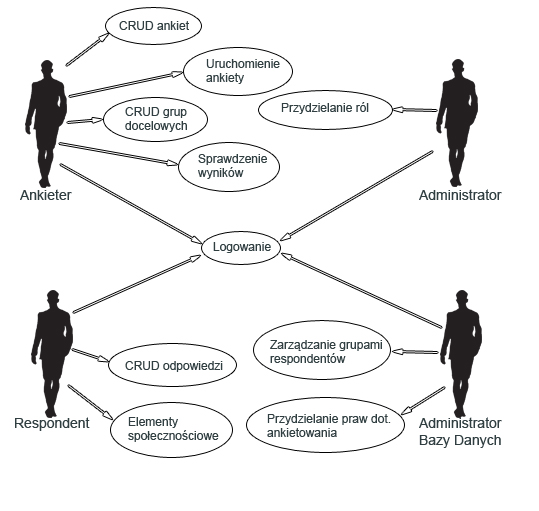
\includegraphics[width=0.9\textwidth]{figures/UseCaseView}
\caption{Diagram przypadków użycia}\label{rys:UseCaseView}
\end{figure}

\section{Ankieter}
\label{Chapter32}

Poniżej przedstawiono przypadki użycia dotyczące Ankietera.

\subsection{UC01: Stworzenie Ankiety}
\label{Chapter321}

\ucsection{UC01: Stworzenie Ankiety}{Ankieter}
{Ankieter jest zalogowany w Systemie i chce utworzyć Ankietę}
{}{\ucactions{
\ucaction{1. Ankieter uruchamia interfejs tworzenia Ankiety. Podaje atrybuty Ankiety: nazwę Ankiety, wstęp, podsumowanie}
\ucaction{2. System prezentuje stronę umożliwiającą dodawanie pytań}
\ucaction{3. Ankieter wybiera typ pytania}
\ucaction{4. Ankieter podaje treść pytania}
\ucaction{5. Ankieter podaje możliwe odpowiedzi}
\ucaction{6. Ankieter akceptuje Ankietę}
\ucaction{7. System prezentuje podsumowanie ankiety i zapisuje ją w Katalogu Ankiet ankietera}
}}
{\ucextensions{
\ucaction{4.A Typ pytania: pytanie otwarte}
\ucaction{4.A.1 Ankieter pomija krok 5.}
\ucaction{6.A Ankieter chce dodać kolejne pytanie}
\ucaction{6.A.1 Powrót do kroku 3.}
}}
{}

\subsection{UC02: Edycja Ankiety}
\label{Chapter322}

\ucsection{UC02: Edycja Ankiety}{Ankieter}
{
1. Ankieta znajduje się w Systemie i jest dostępna dla Ankietera \\
2. Ankieta nie jest częścią czynnego Badania \\
3. Ankieter jest zalogowany w Systemie i chce zmodyfikować istniejącą Ankietę
}
{}{\ucactions{
\ucaction{1. Ankieter wybiera Ankietę do modyfikacji}
\ucaction{2. System prezentuje wskazaną Ankietę}
\ucaction{3. Ankieter modyfikuje lub usuwa dostępne pytania}
\ucaction{4. Ankieter potwierdza chęć zapisu zmienionej Ankiety}
\ucaction{5. System zapisuje zmienioną Ankietę}
}}
{\ucextensions{
\ucaction{3.A. Edycja możliwych odpowiedzi do pytań}
\ucaction{3.A.1 Ankieter edytuje możliwe odpowiedzi do pytań}
}}
{}

\subsection{UC03: Wybór Grupy Docelowej}
\label{Chapter323}

\ucsection{UC03: Wybór Grupy Docelowej}{Ankieter, Administrator}
{
1. Ankieta znajduje się w Systemie i jest dostępna dla Ankietera \\
2. Grupa Docelowa znajduje się w Systemie i jest dostępna dla Ankietera \\
3. Ankieter jest zalogowany w Systemie i chce wybrać Grupę Docelową
}
{}{\ucactions{
\ucaction{1. Ankieter wybiera opcję tworzenia Badania}
\ucaction{2. System prezentuje listę Grup Docelowych, do których Ankieter ma uprawnienia}
\ucaction{3. Ankieter wybiera Grupy Docelowe dla danego Badania}
\ucaction{4. Ankieter akceptuje powiązanie Grup Docelowych z Ankietą}
}}
{\ucextensions{
\ucaction{3.A. Zawężenie Grupy Docelowej}
\ucaction{3.A.1 Ankieter wybiera członków Grupy Docelowej, do której ma być skierowana Ankieta.}
\ucaction{3.A.2 Powrót do kroku 4.}
\ucaction{3.B. Grupa Docelowa poszukiwana przez Ankietera nie istnieje}
\ucaction{3.B.1 Ankieter próbuje połączyć kilka Grup Docelowych lub ich fragmentów}
\ucaction{3.B.2 W przypadku niepowodzenia kroku rozszerzenia 3.B.1, bądź wystąpienia takiej konieczności, Ankieter informuje Administratora, że nie ma praw do wysyłania ankiet do wskazanych osób i/lub powiadamia go (za pomocą poczty elektronicznej) o potrzebie stworzenia Grupy Docelowej o konkretnych atrybutach (BC03)}
\ucaction{3.B.3 W przypadku pominięcia kroku rozszerzenia 3.B.2, powrót do kroku 4., w przeciwnym razie, powrót do kroku 1.}
}}
{}

\subsection{UC04: Uruchomienie Badania}
\label{Chapter324}

\ucsection{UC04: Uruchomienie Badania}{Ankieter, Respondent}
{
1. Ankieta znajduje się w Systemie i jest dostępna dla Ankietera \\
2. Ankieta jest powiązana z Grupą Docelową \\
3. Ankieter jest zalogowany w Systemie i chce rozesłać istniejącą Ankietę
}
{Respondenci powiadomieni o Ankiecie}{\ucactions{
\ucaction{1. Ankieter ustawia czas rozpoczęcia i zakończenia Badania oraz grupę docelową (UC3)}
\ucaction{2. Ankieter potwierdza chęć uruchomienia Badania}
\ucaction{3. System udostępnia Ankietę Respondentom}
\ucaction{4. System powiadamia Respondentów o Ankiecie}
}}
{\ucextensions{
\ucaction{1.A. Ankieter chce prowadzić cykliczną ankietyzację}
\ucaction{1.A.1 Ankieter ustawia częstotliwość powtarzania Badania}
}}
{}

\subsection{UC06: Sprawdzenie wyników}
\label{Chapter325}

\ucsection{UC06: Sprawdzenie wyników}{Ankieter}
{
1. Ankieta znajduje się w Systemie, zawiera odpowiedzi od Grupy Docelowej i jest dostępna dla Ankietera \\
2. Ankieter jest zalogowany w Systemie i chce pozyskać informacje od Studentów/Absolwentów
}
{Wygenerowany Raport}{\ucactions{
\ucaction{1. Ankieter wybiera Ankietę, której wyniki chce poznać}
\ucaction{2. Ankieter wybiera typ Raportu, który chciałby zobaczyć}
\ucaction{3. System generuje i wyświetla Raport}
}}
{}

\section{Respondent}
\label{Chapter33}

Poniżej przedstawiono przypadki użycia dotyczące Respondenta.

\subsection{UC05: Udzielenie odpowiedzi}
\label{Chapter331}

\ucsection{UC05: Udzielenie odpowiedzi}{Respondent}
{
1. Respondent dostaje powiadomienie o Ankiecie (link bezpośredni do Ankiety) \\
2. Respondent jest zalogowany w Systemie i chce wypełnić Ankietę
}
{}{\ucactions{
\ucaction{1. Respondent wybiera Ankietę, w której chce wziąć udział}
\ucaction{2. System prezentuje wybraną Ankietę Respondentowi}
\ucaction{3. Respondent udziela odpowiedzi na pytania}
\ucaction{4. Respondent zatwierdza wypełnioną Ankietę}
\ucaction{5. System zapisuje odpowiedzi}
}}
{\ucextensions{
\ucaction{2.A. Przedawniona Ankieta}
\ucaction{2.A.1 System informuje, że Ankieta już się zakończyła}
\ucaction{5.A. Brak odpowiedzi na niektóre pytania}
\ucaction{5.A.1 System pozwala powrócić do pytań, na które nie udzielono odpowiedzi}
\ucaction{5.A.2 Powrót do kroku 1.}
}}
{}

\section{Administrator}
\label{Chapter34}

Poniżej przedstawiono przypadki użycia dotyczące Administratora.

\subsection{UC07: Tworzenie Grupy Docelowej}
\label{Chapter341}

\ucsection{UC07: Tworzenie Grupy Docelowej}{Administrator}
{
1. Ankieter chce wysyłać Ankiety do określonych Respondentów w prosty sposób \\
2. Administrator jest zalogowany w Systemie i chce utworzyć nową Grupę Docelową
}
{Nowa Grupa Docelowa w Systemie}{\ucactions{
\ucaction{1. Administrator wybiera opcję tworzenia Grup Docelowych}
\ucaction{2. System prezentuje formularz tworzenia Grupy Docelowej}
\ucaction{3. Administrator wprowadza nazwę tworzonej Grupy Docelowej, wybiera Grupę Nadrzędną oraz Respondentów do dodania do Grupy Docelowej}
\ucaction{4. Administrator potwierdza chęć stworzenia Grupy Docelowej}
\ucaction{5. System zapisuje nową Grupę Docelową}
}}
{\ucextensions{
\ucaction{4.A Brak Grupy Nadrzędnej}
\ucaction{4.A.1 Administrator Bazy Danych nie uzupełnia Grupy Nadrzędnej}
}}
{}

\subsection{UC08: Edycja Grupy Docelowej}
\label{Chapter342}

\ucsection{UC08: Edycja Grupy Docelowej}{Administrator}
{
1. Grupa Docelowa znajduje się w Systemie \\
2. Administrator jest zalogowany w Systemie i chce zmodyfikować Grupę Docelową
}
{Zmodyfikowana lista członków Grupy Docelowej}{\ucactions{
\ucaction{1. Administrator wybiera Grupę Docelową}
\ucaction{2. Administrator wybiera członka\slash członków Grupy Docelowej do edycji\slash usunięcia}
\ucaction{3. Administrator dodaje\slash edytuje]\slash usuwa członka\slash członków Grupy Docelowej}
\ucaction{4. Administrator potwierdza chęć wprowadzenia zmian}
\ucaction{5. System zapisuje zmiany}
}}
{}

\section{Wszyscy Użytkownicy}
\label{Chapter35}

Poniżej przedstawiono przypadki użycia dotyczące wszystkich Użytkowników.

\subsection{UC09: Logowanie do Systemu}
\label{Chapter351}

\ucsection{UC09: Logowanie do Systemu}{Użytkownik (Ankieter, Administrator, Respondent)}
{Użytkownik posiada konto w Systemie i posiada poprawne dane logowania}
{Użytkownik jest zalogowany w Systemie}{\ucactions{
\ucaction{1. System wyświetla Użytkownikowi formularz logowania}
\ucaction{2. Użytkownik podaje login lub adres e-mail oraz hasło}
\ucaction{3. System uwierzytelnia Użytkownika}
}}
{\ucextensions{
\ucaction{2.A Użytkownik chce się zalogować przy pomocy \textit{eKonta}}
\ucaction{2.A.1 Użytkownik wybiera opcję logowania przez \textit{eKonto}}
\ucaction{2.A.2 System przekierowuje Użytkownika na stronę logowania przez \textit{eKonto} (\textit{eLogin})}
\ucaction{2.A.3 Użytkownik wprowadza dane logowania do \textit{eKonta}}
\ucaction{2.A.4 Powrót do kroku 3.}
}}
{}
\chapter{Wymagania pozafunkcjonalne}
\label{Chapter4}

\section{Wstęp}
\label{Chapter41}

W~niniejszym rozdziale zostaną zaprezentowane i~krótko opisane wymagania pozafunkcjonalne dotyczące systemu \textit{iQuest}. Dodatkowo, zostały one przydzielone do wybranych przez zespół zarządzający charakterystyk oprogramowania.

\section{Opis wymagań}
\label{Chapter42}

Wymagania pozafunkcjonalne przypisane do~wyżej opisanych charakterystyk oprogramowania przedstawione zostały w~tabeli \ref{tab:reqs}. Dodatkowo, określono za~pomocą etykiety \emph{ważność~(W)} oraz~\emph{trudność implementacji~(TI)} dla~każdego z~wymagań. Wartości w~ramach tego oznaczenia wyrażone~są w~następującej skali:

\begin{itemize}
\item{H (ang.~\definicja{high}) -- wysoka}
\item{M (ang.~\definicja{medium}) -- średnia}
\item{L (ang.~\definicja{low}) -- niska}
\end{itemize}

Analizy, zakończonej etykietowaniem, dokonał zespół zarządzający, rozpatrując to~wedle wytycznych przedstawionych w trakcie zajęć akademickich na 1.~roku studiów II~stopnia.

\newpage
\begin{center}
\begin{longtable}{ | p{4cm} | p{9cm} | c | c | }
\hline
\textbf{Charakterystyka} & \textbf{Wymaganie} & \textbf{W} & \textbf{TI} \\ \hline
%
Analizowalność & Komentarze w kodzie źródłowym powinny być w języku angielskim. & M & L \\ \hline
Analizowalność & Kod źródłowy sytemu powinien być utworzony zgodnie ze standardami \textit{Moodle}. & M & L \\ \hline
Analizowalność & System powinien zawierać testy jednostkowe. & M & M \\ \hline
Analizowalność & System powinien rejestrować stack trace i rodzaj błędu (fatal, warning). & H & L \\ \hline
Analizowalność & Wraz z kodem źródłowym systemu należy dostarczyć dokumentację. & H & M \\ \hline
Analizowalność & System powinien logować niewłaściwe wywołania metod. & H & L \\ \hline
%
Autentyczność & Gdy student staje się absolwentem, należy umożliwić mu dalsze logowanie się do systemu bez użycia \textit{eKonta}. & H & M \\ \hline
%
Bezpieczeństwo (wolność od ryzyka) & Dane (opinie respondentów) przechowywane w systemie muszą być uzyskiwane poprzez wbudowane mechanizmy ankietowania. & H & L \\ \hline
Bezpieczeństwo (wolność od ryzyka) & Projekt systemu należy poddać analizie z wykorzystaniem metody ATAM. & M & M \\ \hline
%
Charakterystyka czasowa & Wyświetlenie ankiety powinno trwać nie dłużej niż 4 sekundy. & H & L \\ \hline
Charakterystyka czasowa & Generowanie raportów powinno odbywać się ze średnio nie dłużej niż 1 godzinę. & M & M \\ \hline
Charakterystyka czasowa & Należy zdefiniować klasy operacji, w zależności od czasu ich trwania. Klasy:
\begin{itemize}
\item{bez komunikatu potwierdzającego wykonanie}
\item{z potwierdzeniem wykonania}
\item{wykonywane na serwerze w tle}
\end{itemize} & M & M \\ \hline
%
Dostępność personalna & Przewidzieć, na poziomie architektury, możliwość rozbudowy np. o interfejs dla osób niedowidzących. & L & M \\ \hline
%
Dostępność techniczna & System może mieć przerwę serwisową, lecz musi wówczas prezentować specjalny ekran informujący o czasie jej trwania. & H & L \\ \hline
%
Estetyka Interfejsu Użytkownika & Środowisko ma być przyjazne i czytelne dla użytkownika końcowego. & H & M \\ \hline
%
Funkcjonalna poprawność & Wszystkie wartości mają być prezentowane z dokładnością do 2~miejsc po przecinku. & H & L \\ \hline
%
Identyfikowalność & System ma umożliwiać identyfikowanie podmiotów (osobno: administratorów, ankieterów, respondentów), podejmujących konkretne działania: tworzenie ankiet, odpowiadanie w 
ankietach, itp. & H & M \\ \hline
%
Integralność & Baza danych powinna być chroniona przed nieuprawnionym dostępem [modyfikacją\slash usunięciem] w następujący sposób: logowanie za pomocą loginu i hasła. & H & L \\ \hline
Integralność & System powinien być odporny na następujące próby nielegalnego dostępu: nieuprawniony dostęp fizyczny do serwera. & M & L \\ \hline
Integralność & Należy chronić\slash szyfrować dane przesyłane z i do systemu. & M & L \\ \hline
%
Interoperacyjność & System ma wymieniać potrzebne dane z systemami uczelnianymi: \textit{eKonto}, \textit{eDziekanat}, \textit{ePoczta}. Dane mają być aktualne. & H & M \\ \hline
Interoperacyjność & System ma pobierać dane z systemu \textit{eDziekanat} w następujący sposób: \textit{SOAP}. & H & M \\ \hline
Interoperacyjność & System ma przesyłać dane o wiadomościach do wysłania do systemu \textit{ePoczta} w następujący sposób: \textit{SOAP}. & H & M \\ \hline
Interoperacyjność & System ma pobierać dane do autoryzacji z systemu \textit{eKonto} w następujący sposób: \textit{SOAP}. & H & M \\ \hline
Interoperacyjność & System ma przesyłać wyniki ankiet do systemu \textit{BI}\footnote{ang. \definicja{Business Intelligence}}. & H & M \\ \hline
%
Kompletność kontekstowa & System ma działać w przeglądarkach: \textit{IE 7.0+}, \textit{Firefox 15}, \textit{Opera 12}. & H & M \\ \hline
Kompletność kontekstowa & Należy przygotować raport jak system zachowuje się na platformach mobilnych. & L & L \\ \hline
%
Łatwość adaptacji & Należy utworzyć raport z łatwości adaptacji oraz gdzie znajdują się adaptery. & M & L \\ \hline
%
Łatwość instalacji & System musi umożliwiać łatwą aktualizacje, przy założeniu, że wersja platformy \textit{Moodle} pozostaje bez zmian. & H & H \\ \hline
%
Łatwość nauczenia się & Interfejs użytkownika (dla ankietowanych) powinien być całkowicie intuicyjny. & H & M \\ \hline
Łatwość nauczenia się & Interfejs użytkownika (dla ankietera) może wymagać nieznacznego doszkolenia obsługujących. & M & L \\ \hline
%
Łatwość testowania & ,,Atrapy'' (ang.~\definicja{mock}) systemów zewnętrznych (m.in. \textit{eKonto}, \textit{ePoczta}). & M & M \\ \hline
Łatwość zamiany & Należy umożliwić przełączanie systemu między trybem testowym i produkcyjnym. & M & L \\ \hline
%
Łatwość zamiany & System powinien umożliwiać wczytanie wszystkich danych z poprzedniej wersji. & H & M \\ \hline
Łatwość zamiany & Procedura wymiany oprogramowania powinna trwać nie dłużej niż 2 dni i odbywać się w następujący sposób: zgodność z instrukcją. & M & L \\ \hline
Łatwość zamiany & Podczas projektowania systemu, należy brać pod uwagę możliwość wprowadzenia wielojęzyczności interfejsu. & M & M \\ \hline
%
Łatwość zmiany & System powinien być przygotowany na wprowadzenie następujących zmian: nowe typy raportów, nowe typy pytań, modyfikacje interfejsów systemów zewnętrznych. & M & M \\ \hline
%
Niezaprzeczalność & System musi posiadać logi (zalogowanie w systemie, stworzenie\slash edycja\slash usunięcie\slash wysłanie\slash wypełnienie ankiety), aby móc udokumentować skąd pochodzą dane. & H & L \\ \hline
%
Ochrona użytkownika przed błędami & Dodatkowe potwierdzenie chęci wykonania operacji nieodwracalnych (nawet dla administratora), lub możliwość przywrócenia usuniętych danych przez jakiś czas. & H & M \\ \hline
Ochrona użytkownika przed błędami & Dla dużych ankiet, zatwierdzenie odesłania jej przez ankietowanego. & M & L \\ \hline
Ochrona użytkownika przed błędami & Potwierdzenie przed rozesłaniem ankiet. & M & L \\ \hline
Ochrona użytkownika przed błędami & Lista operacji wykonywanych w tle. & M & L \\ \hline
%
Odporność na wady & Gdy nastąpi awaria innych systemów np. \textit{eKonto}, należy poinformować użytkownika o błędzie i uniemożliwić mu dalsze działanie w systemie. & H & L \\ \hline
%
Odtwarzalność & Odtwarzanie całego systemu w czasie nieprzekraczającym 3h. & M & L \\ \hline
Odtwarzalność & Kopia zapasowa bazy danych wykonywana z częstotliwością raz na dobę. & H & L \\ \hline
Odtwarzalność & Dostępność instrukcji odtwarzania. & H & L \\ \hline
Odtwarzalność & Wykonywanie operacji w transakcjach tam, gdzie to możliwe. & H & L \\ \hline
%
Poufność & Uwierzytelnianie i autoryzacja dla każdej operacji. & M & L \\ \hline
%
Współistnienie & Jedynym kryterium działania systemu ankiet (bez raportów) jest działająca przeglądarka. & H & L \\ \hline
Współistnienie & System generowania raportów może być osobną aplikacją, działającą na specjalnych: sprzęcie i oprogramowaniu. & L & L \\ \hline
Współistnienie & Wszystkie potrzebne dane z zewnętrznych systemów należy przechowywać lokalnie i synchronizować. & M & H \\ \hline
Współistnienie & Należy kolejkować zadania (np.~e-maile) w systemie, na czas braku możliwości ich wysłania (np.~awaria \textit{ePoczty}). & H & M \\ \hline
%
Zużycie zasobów & System nie powinien wykorzystywać więcej serwerów \textit{HTTP} niż jeden. & M & L \\ \hline
Zużycie zasobów & System powinien działać poprawnie przy nawet 10.000 użytkowników zalogowanych jednocześnie. & H & M \\ \hline
Zużycie zasobów & Zadania, które nie muszą zostać wykonane natychmiastowo, powinny być kolejkowane przez system. & M & M \\ \hline
Zużycie zasobów & Możliwość pracy przez ankietera\slash respondenta na średniej klasy laptopie (CPU 2GHz, RAM 4GB). & H & L \\ \hline
%
\caption{Wymagania pozafunkcjonalne}\label{tab:reqs}
\end{longtable}
\end{center}

Zważywszy, że~projekt ten jest istotny dla~Uczelni, dołożono wszelkich starań, aby~spełnić wszystkie wymagania pozafunkcjonalne. Zadanie to~zostało w~sporej części wykonane dzięki zastosowaniu sprawdzonego i~znanego narzędzia w~roli podstawy dla~całego~systemu. Mowa o platformie \textit{Moodle}\footnote{Więcej informacji w~rozdziale~\ref{Chapter6}, poświęconym implementacji i~zastosowanym przy~niej technologiom.}. Użycie jej~pozwoliło m.in.~na~zapewnienie modułowości systemowi. Spełniona została także adaptatywność i~przenośność systemu, oparta na~uniwersalności języka \textit{PHP}, jak~też szerokiej gamie obsługiwanych przez~\textit{Moodle} systemów baz~danych. \\

Zalety wykorzystania tak~powszechnej technologii były -- przynajmniej w teorii -- znacznie szersze. \textit{Moodle} posiada swój własny standard kodowania, którego~przy realizowaniu projektu starano~się w~pełni przestrzegać. To sprawia, że~w~połączeniu z wytycznymi \textit{DRO} (\definicja{Dział Rozwoju Oprogramowania Politechniki Poznańskiej}), dokumentacją \textit{Moodle} i~dokumentacją systemu \textit{iQuest}, nakład pracy wymagany do~wdrożenia~się, w~celu rozwoju projektu, został zmniejszony. \\

W~trakcie prac nad projektem, niemały nacisk stawiano na~prawidłowe zarządzanie uprawnieniami użytkowników. Wykorzystano w~tym celu mechanizmy dostępne w~platformie \textit{Moodle}. Są one weryfikowane przy każdym działaniu podejmowanym przez użytkowników i~zależą od~przydzielonej im~w~systemie roli. Szczegóły tej~kwestii swobodnie definiować może administracja. Ważnym jest, że~osoby pełniące rolę ankietera mogą modyfikować i~analizować jedynie te badania, które zostały utworzone przez~siebie lub~udostępnione im~bezpośrednio. Podobnie działają uprawnienia przydzielone do~roli respondenta -- pozwalając dokładnie jeden~raz odpowiedzieć na~pytania w~ankietach skierowanych do~grup docelowych, do~których należy użytkownik.
\chapter{Architektura systemu}
\label{Chapter5}

\section{Wstęp}
\label{Chapter51}

System \textit{iQuest} został stworzony w oparciu o model architektury trójwarstwowej, w którym wyróżnione zostały warstwy: danych, logiki biznesowej oraz prezentacji. Dzięki takiemu podejściu, zadania związane z poszczególnymi warstwami można było bez większego problemu rozdzielić między członków zespołu programistów, a w przypadku ewentualnej modyfikacji jednej z warstw nie występuje konieczność wprowadzania zmian w reszcie projektu.

\section{Opis ogólny architektury -- ,,Marketektura''}
\label{Chapter52}

System \textit{iQuest} to aplikacja internetowa w postaci zbioru rozszerzeń platformy e-learningowej \textit{Moodle}. Całość (\textit{Moodle} oraz rozszrzenia) zainstalowana jest na serwerze www, zlokalizowanym w sieci Politechniki Poznańskiej, łączącym się z osobnym serwerem baz danych oraz usługami \textit{eKonto} i \textit{eDziekanat}. Funkcje raportowania realizowane są w głównej mierze za pośrednictwem zewnętrznego systemu \textit{BI}, pobierającego dane z \textit{iQuest} za pośrednictwem usług sieciowych (ang.~\definicja{webservices}). Administracja oraz obsługa systemu odbywa się za pośrednictwem przeglądarki internetowej, w ramach połączenia z platformą \textit{Moodle} lub serwerem raportowania. Respondenci mogą też uzyskać dostęp do systemu przy pomocy urządzeń mobilnych, takich jak tablety czy smartfony.

\begin{figure}[H]
\centering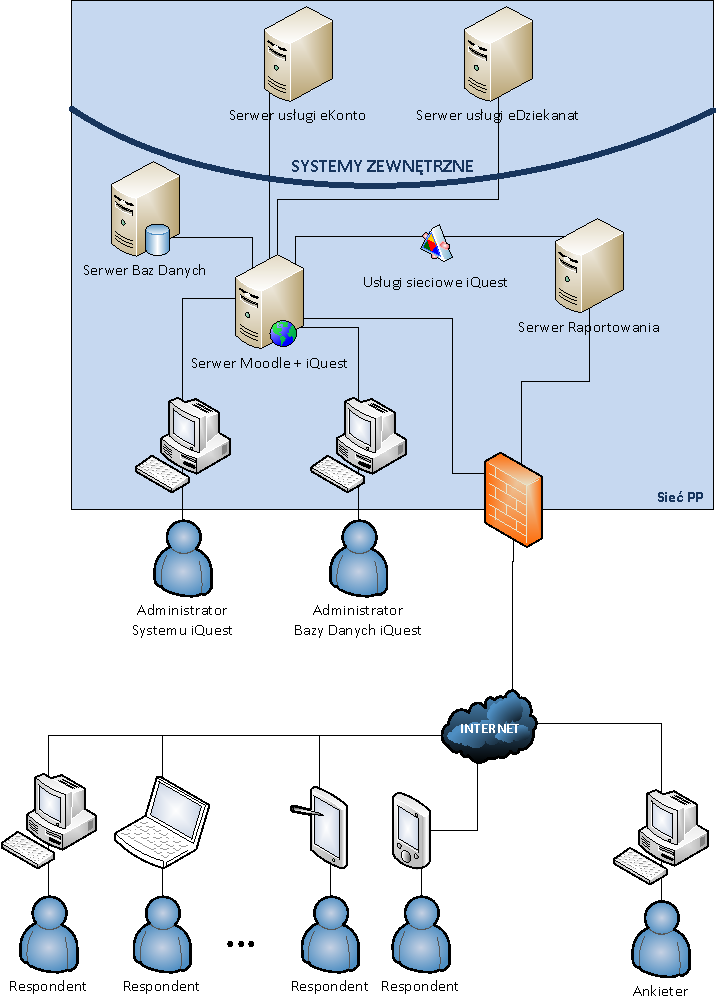
\includegraphics[width=0.9\textwidth]{figures/marketecture}
\caption{Diagram ,,Marketektury''}\label{rys:marketecture}
\end{figure}

\section{Analiza~podejść\slash Analiza~SWOT}
\label{Chapter53}

W fazie inicjacji projektu, zespół zarządzający przeprowadził analizę SWOT (ang. \definicja{Strengths, Weaknesses, Opportunities, Threats} - mocne strony, słabe strony, szanse, zagrożenia). Poniżej zamieszczono tabele \ref{tab:SWOT1}. oraz \ref{tab:SWOT2}., zawierające jej wyniki. W oparciu o nie, zespół zarządzający podjął decyzję o realizacji projektu z użyciem platformy \textit{Moodle}.

\begin{table}[H]
\centering
\begin{tabular}{ | p{2.5cm} | p{5.5cm} | p{5.5cm} | }
\hline
--- & \textbf{Pozytywne} & \textbf{Negatywne} \\ \hline
\multirow{6}{*}{\textbf{Wewnętrzne}} & \textbf{Mocne strony (S)} & \textbf{Słabe strony (W)} \\
			& Środowisko \textit{Moodle} jest dobrze udokumentowane\cite{Man:Moodle}. & Konieczność trzymania się standardów \textit{Moodle}. \\
			& Środowisko \textit{Moodle} jest łatwe w rozwoju. & Konieczność wdrożenia się w nieznany kod. \\
			& Stosowanie podejścia MVC w środowisku \textit{Moodle}. & \\
			& Już zaimplementowane mechanizmy, takie jak kontrola praw dostępu, CMS. & \\
			& Posiadanie bazy wiedzy, która ma zachęcać użytkowników. & \\ \hline
%					
\multirow{3}{*}{\textbf{Zewnętrzne}} & \textbf{Szanse (O)} & \textbf{Zagrożenia (T)} \\
				& Modułowość platformy \textit{Moodle}. & Środowisko może być nieznane programistom. \\
				& Łatwość tworzenia własnych wtyczek. & \\ \hline
\end{tabular}
\caption{Podejście pierwsze -- w oparciu o platformę \textit{Moodle}}\label{tab:SWOT1}
\end{table}

\begin{table}[H]
\centering
\begin{tabular}{ | p{2.5cm} | p{5.5cm} | p{5.5cm} | }
\hline
--- & \textbf{Pozytywne} & \textbf{Negatywne} \\ \hline
\multirow{2}{*}{\textbf{Wewnętrzne}} & \textbf{Mocne strony (S)} & \textbf{Słabe strony (W)} \\
			& Dostępność platformy na wszystkich popularnych systemach operacyjnych. & Konieczność implementacji dodatkowych funkcjonalności związanych z zachęcaniem do korzystania z systemu. \\ \hline
%					
\multirow{3}{*}{\textbf{Zewnętrzne}} & \textbf{Szanse (O)} & \textbf{Zagrożenia (T)} \\
				& Dobra znajomość kodu przez programistów. & Konieczność tworzenia wszystkiego od podstaw. \\
				& & Nieznajomość technologii przez programistów. \\ \hline
\end{tabular}
\caption{Podejście drugie -- napisanie aplikacji od podstaw przy użyciu \textit{Java~EE}}\label{tab:SWOT2}
\end{table}

Rozpatrując powyższe tabele z perspektywy czasu, autorzy niniejszej pracy stwierdzili, iż analiza SWOT została zrealizowana nieprawidłowo, faworyzując rozwiązanie z użyciem systemu \textit{Moodle}. Dla przykładu, dokumentacja \textit{Moodle} okazała się być w znacznym stopniu nieprecyzyjna i niekompletna, zaś w kodzie platformy nie stosuje się podejścia MVC.

\section{Perspektywy architektoniczne}
\label{Chapter54}

\subsection{Perspektywa fizyczna}
\label{Chapter541}

\begin{figure}[H]
\centering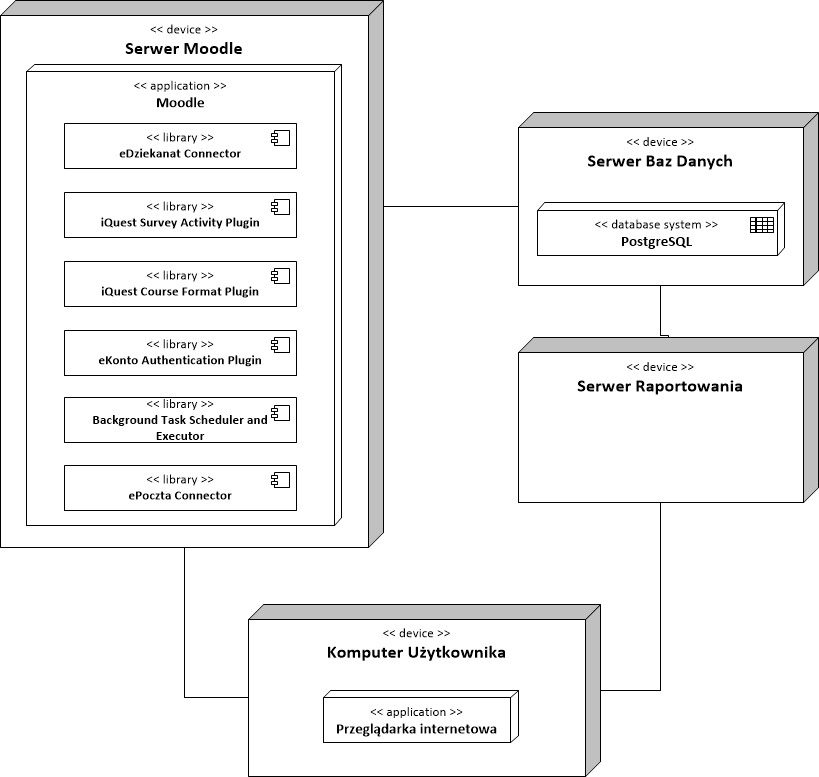
\includegraphics[width=0.9\textwidth]{figures/PhysicalView}
\caption{Diagram perspektywy fizycznej}\label{rys:PerspektywaFizyczna}
\end{figure}

Schemat \ref{rys:PerspektywaFizyczna} prezentuje perspektywę fizyczną projektu. Widać na nim dokładnie, opisaną wcześniej, opartą na rozszerzeniach dla platformy \textit{Moodle} budowę logiki systemu \textit{iQuest}. Za jej pośrednictwem dokonuje się połączeń z serwerem baz danych oraz serwerem raportowania. Użytkownik systemu, z wykorzystaniem przeglądarki internetowej, komunikuje się z platformą, lub systemem raportowania, korzystając przy tym z warstwy prezentacji.

\subsection{Perspektywa logiczna}
\label{Chapter542}

\begin{figure}[H]
\centering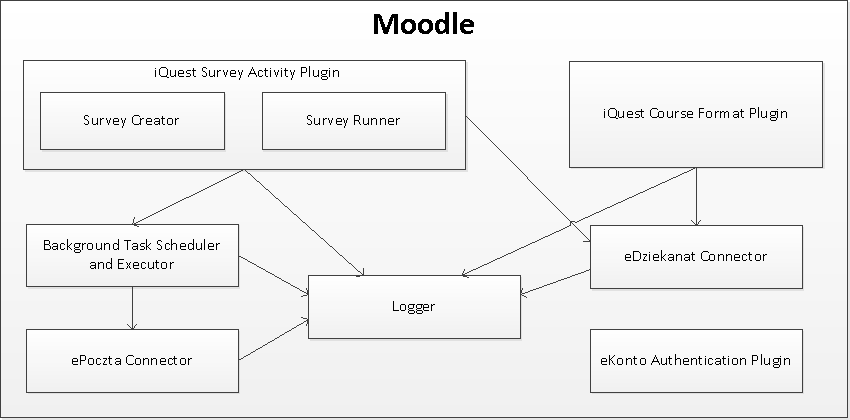
\includegraphics[width=0.9\textwidth]{figures/LogicalView}
\caption{Diagram perspektywy logicznej}\label{rys:PerspektywaLogiczna}
\end{figure}

Schemat \ref{rys:PerspektywaLogiczna} prezentuje perspektywę logiczną systemu. Określa ona zależności między poszczególnymi komponentami ,,wszczepionymi'' do platformy \textit{Moodle}. Poniżej znajduje się opis wyszczególnionych na rysunku komponentów.

\subsubsection{iQuest Survey Activity Plugin}
\label{Chapter5421}
Funkcjonalnością \definicja{Activity Plugin} jest udostępnianie możliwości dodania nowych rodzajów tzw. ,,aktywności'' w ramach platformy \textit{Moodle}. \textit{iQuest Survey Activity Plugin} pozwala na dodanie nowego badania \textit{iQuest}. Komponent ten składa się z dwóch subkomponentów:
\begin{itemize}
\item{Survey Creator}
\item{Survey Runner}
\end{itemize}
Pierwszy z nich odpowiada za definiowanie ankiet, natomiast drugi za ich realizację.

\subsubsection{iQuest Course Format Plugin}
\label{Chapter5422}

\definicja{Course Format Plugin} dla platformy \textit{Moodle} odpowiada za obsługę interfejsu użytkownika. W przypadku systemu \textit{iQuest}, zarządza kwestią wyświetlania użytkownikowi tylko tych składowych kursu związanego z systemem \textit{iQuest}, które są dla niego dostępne. Przykładowo, Respondent uzyska dostęp do listy ankiet, które może wypełnić, podczas gdy ankieter uzyska dostęp do listy zarządzanych przez niego badań.

\subsubsection{eDziekanat Connector oraz ePoczta Connector}
\label{Chapter5423}

Komponenty te odpowiadają za komunikację z usługami \textit{eDziekanat} i \textit{ePoczta}, pozwalające m.in. na pozyskanie danych o grupach docelowych (w oparciu o dane Grup Dziekańskich) oraz wysyłanie powiadomień za pośrednictwem poczty studenckiej.

\subsubsection{Background Task Scheduler and Executor}
\label{Chapter5424}

Dzięki temu komponentowi możliwe jest szeregowanie oraz wykonywanie zadań w tle. Jednym z jego zadań jest kolejkowanie i aktywowanie mechanizmów rozsyłania wiadomości e-mail z zaproszeniami do udziału w ankiecie.

\subsubsection{eKonto Authentication Plugin}
\label{Chapter5425}

\definicja{eKonto Authentication Plugin} -- to moduł uwierzytelniania (ang.~\definicja{Authentication}), korzystający z systemu \textit{eLogin} platformy \textit{eKonto} do logowania się do platformy \textit{Moodle}, obsługującej system \textit{iQuest}. Korzystanie z tego systemu pozwala nie tylko na jednoznaczną weryfikację tożsamości użytkownika łączącego się z systemem, ale jest zarazem wygodne -- dzięki jego zastosowaniu, nie ma potrzeby posiadania osobnego konta w systemie \textit{iQuest}.

\subsection{Perspektywa implemetancyjna}
\label{Chapter543}

\begin{figure}[H]
\centering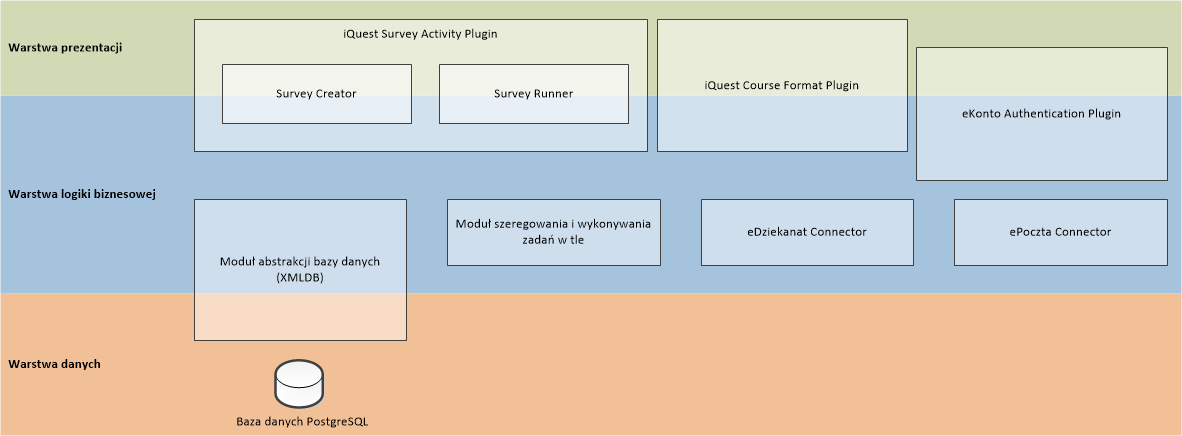
\includegraphics[width=0.9\textwidth]{figures/Layers}
\caption{Diagram perspektywy implementacyjnej}\label{rys:PerspektywaImplementacyjna}
\end{figure}

Diagram perspektywy implementacyjnej (rys.~\ref{rys:PerspektywaImplementacyjna}) pozwala na analizę przeplatania się elementów systemu \textit{iQuest} w ramach poszczególnych warstw zastosowanego modelu trójwarstwowego. Funkcje zaprezentowanych na nim modułów zostały wyjaśnione już wcześniej w niniejszym dokumencie.

\section{Decyzje projektowe}
\label{Chapter55}

\subsection{Wstęp}
\label{Chapter551}

W procesie rozwoju systemu \textit{iQuest} podjęto dokładnie 40 decyzji projektowych. Większość decyzji podejmował Architekt. W części przypadków rozpatrywano także zdanie zespołu programistów.

\subsection{Podjęte decyzje}
\label{Chapter552}

%1
\begin{table}[H]
\centering
\begin{tabular}{ | >{\bfseries}c | p{11cm} | }
\hline
%
Identyfikator & D01 \\ \hline
Nazwa & Postać systemu \\ \hline
Opis & System iQuest jest zestawem rozszerzeń środowiska \textit{Moodle} \\ \hline
Uzasadnienie & Platforma \textit{Moodle} jest już stosowana na uczelni, więc łatwiej jest dotrzeć z ankietami do studentów, jeżeli można je wypełniać bezpośrednio w \textit{Moodle'u}. \\ \hline
Źródło & Architekt \\ \hline
%
\end{tabular}
\end{table}

%2
\begin{table}[H]
\centering
\begin{tabular}{ | >{\bfseries}c | p{11cm} | }
\hline
%
Identyfikator & D02 \\ \hline
Nazwa & Podział na komponenty  \\ \hline
Opis & \textit{iQuest} składa się z następujących głównych komponentów: \textit{iQuest Course Format Plugin}, \textit{iQuest Survey Activity Plugin}, \textit{eDziekanat Connector}, \textit{eKonto Authentication Plugin}, \textit{Background Task Scheduler and Executor}, \textit{Logger}  \\ \hline
Uzasadnienie & Dzięki budowie modułowej łatwiej jest analizować, implementować i testować system. \\ \hline
Źródło & Architekt \\ \hline
%
\end{tabular}
\end{table}

%3
\begin{table}[H]
\centering
\begin{tabular}{ | >{\bfseries}c | p{11cm} | }
\hline
%
Identyfikator & D03 \\ \hline
Nazwa & \textit{iQuest} jako kurs na \textit{Moodle'u}  \\ \hline
Opis & \textit{iQuest} widoczny jest dla użytkowników platformy \textit{Moodle} jako specjalny kurs. \\ \hline
Uzasadnienie & Jest to zgodne z ideą \textit{Moodle'a} -- treści umieszczane na tej platformie są pogrupowane w kursach. \\ \hline
Źródło & Architekt \\ \hline
%
\end{tabular}
\end{table}

%4
\begin{table}[H]
\centering
\begin{tabular}{ | >{\bfseries}c | p{11cm} | }
\hline
%
Identyfikator & D04 \\ \hline
Nazwa & Wtyczka \textit{iQuest Course Format Plugin}  \\ \hline
Opis & \textit{iQuest Course Format Plugin} odpowiada za prezentowanie treści wewnątrz kursu, w ramach którego funkcjonuje system \textit{iQuest}. Plugin dba o to, aby ankieterowi wyświetlała się lista tylko tych badań, do których ma on uprawnienia oraz żeby respondent widział listę tylko tych badań, w których ma on prawo wypełnić ankietę. \\ \hline
Uzasadnienie & Istnienie takiej wtyczki jest wymagane, ponieważ bez niej nie byłoby możliwe filtrowanie listy badań tak, aby użytkownik wydział tylko te do których ma uprawnienia. \\ \hline
Źródło & Architekt \\ \hline
%
\end{tabular}
\end{table}

%5
\begin{table}[H]
\centering
\begin{tabular}{ | >{\bfseries}c | p{11cm} | }
\hline
%
Identyfikator & D05 \\ \hline
Nazwa & \textit{Wtyczka eKonto Authentication Plugin}  \\ \hline
Opis & Logowanie użytkowników przy pomocy \textit{eKonta} realizowane jest poprzez utworzenie rozszerzenia \textit{eKonto Authentication Plugin} dla platformy \textit{Moodle}. \\ \hline
Uzasadnienie & Platforma \textit{Moodle} jest tak skonstruowana, że aby umożliwić uwierzytelnianie przy pomocy zewnętrznych mechanizmów, konieczne jest utworzenie specjalnej wtyczki. \\ \hline
Źródło & Architekt \\ \hline
%
\end{tabular}
\end{table}

%6
\begin{table}[H]
\centering
\begin{tabular}{ | >{\bfseries}c | p{11cm} | }
\hline
%
Identyfikator & D06 \\ \hline
Nazwa & Wtyczka \textit{iQuest Survey Activity Plugin} - funkcjonalność dla ankieterów  \\ \hline
Opis & \textit{iQuest Survey Activity Plugin} pozwala ankieterowi na tworzenie, edytowanie i usuwanie ankiet, a także na tworzenie, edytowanie i usuwanie badań. \\ \hline
Uzasadnienie & Wtyczka typu \textit{Activity Plugin} dla \textit{Moodle'a} posiada wszystkie cechy potrzebne do zrealizowania tego typu funkcjonalności w sposób intuicyjny dla użytkownika. \\ \hline
Źródło & Architekt \\ \hline
%
\end{tabular}
\end{table}

%7
\begin{table}[H]
\centering
\begin{tabular}{ | >{\bfseries}c | p{11cm} | }
\hline
%
Identyfikator & D07 \\ \hline
Nazwa & Wtyczka \textit{iQuest Survey Activity Plugin} - funkcjonalność dla respondentów \\ \hline
Opis & \textit{iQuest Survey Activity Plugin} pozwala respondentowi na udzielenie odpowiedzi w ankiecie. \\ \hline
Uzasadnienie & Wtyczka typu \textit{Activity Plugin} dla \textit{Moodle'a} posiada wszystkie cechy potrzebne do zrealizowania tego typu funkcjonalności w sposób intuicyjny dla użytkownika. \\ \hline
Źródło & Architekt \\ \hline
%
\end{tabular}
\end{table}

%8
\begin{table}[H]
\centering
\begin{tabular}{ | >{\bfseries}c | p{11cm} | }
\hline
%
Identyfikator & D08 \\ \hline
Nazwa & Wykorzystanie protokołu HTTPS \\ \hline
Opis & \textit{Moodle} (w ramach którego działa \textit{iQuest}) będzie dostępny dla użytkowników poprzez protokół HTTPS. \\ \hline
Uzasadnienie & Zastosowanie protokołu HTTPS jest łatwym sposobem na dość skuteczne zabezpieczenie danych przesyłanych między klientem a serwerem. \\ \hline
Źródło & Architekt \\ \hline
%
\end{tabular}
\end{table}

%9
\begin{table}[H]
\centering
\begin{tabular}{ | >{\bfseries}c | p{11cm} | }
\hline
%
Identyfikator & D09 \\ \hline
Nazwa & Mechanizm kont i ról użytkowników \\ \hline
Opis & Wykorzystany jest istniejący w systemie \textit{Moodle} mechanizm kont i ról użytkowników. \\ \hline
Uzasadnienie & Dzięki temu nie ma potrzeby implementowania osobnego mechanizmu. Ten istniejący w \textit{Moodle'u} spełnia niezbędne wymagania. \\ \hline
Źródło & Architekt \\ \hline
%
\end{tabular}
\end{table}

%10
\begin{table}[H]
\centering
\begin{tabular}{ | >{\bfseries}c | p{11cm} | }
\hline
%
Identyfikator & D10 \\ \hline
Nazwa & Integracja \textit{eKonta} z kontem na \textit{Moodle'u} \\ \hline
Opis & W momencie pierwszego logowania danego użytkownika przy pomocy \textit{eKonta}, jest mu tworzone profil w systemie \textit{Moodle}. Za nazwę użytkownika przyjmuje się adres e-mail. Do profilu, dzięki możliwościom usługi \textit{eKonto} kopiowane są także inne dane użytkownika (np. imię i nazwisko). \\ \hline
Uzasadnienie & Takie działanie jest wymagane, aby zainicjalizować konto użytkownika logującego się do \textit{Moodle'a} przez \textit{eKonto} po raz pierwszy. \\ \hline
Źródło & Architekt \\ \hline
%
\end{tabular}
\end{table}

%11
\begin{table}[H]
\centering
\begin{tabular}{ | >{\bfseries}c | p{11cm} | }
\hline
%
Identyfikator & D11 \\ \hline
Nazwa & Sposób zapamiętywania ustawień systemu \textit{iQuest}  \\ \hline
Opis & Ustawienia systemu \textit{iQuest} przechowywane są w specjalnej tabeli bazy danych, w postaci identyfikator-wartość, które są ciągami znaków. \\ \hline
Uzasadnienie & Umożliwia to łatwy i wygodny dostęp do ustawień w różnych miejscach kodu źródłowego systemu. \\ \hline
Źródło & Architekt \\ \hline
%
\end{tabular}
\end{table}

%12
\begin{table}[H]
\centering
\begin{tabular}{ | >{\bfseries}c | p{11cm} | }
\hline
%
Identyfikator & D12 \\ \hline
Nazwa & Dziennik zdarzeń \\ \hline
Opis & Wszystkie ważniejsze zdarzenia w systemie \textit{iQuest} są zapisywane w logu w bazie danych, w specjalnej tabeli. Dla każdego zdarzenia zapisane zostaną następujące dane: data i godzina, identyfikator użytkownika wykonującego operację (o ile dotyczy), tekstowy opis, typ (informacja, ostrzeżenie, błąd). \\ \hline
Uzasadnienie & Mechanizm logowania zdarzeń obecny w \textit{Moodle'u} nie spełnia wymagań - nie pozwala na dzielenie wpisów na kategorie. Z tego powodu została podjęta decyzja o utworzeniu osobnego mechanizmu. \\ \hline
Źródło & Architekt \\ \hline
%
\end{tabular}
\end{table}

%13
\begin{table}[H]
\centering
\begin{tabular}{ | >{\bfseries}c | p{11cm} | }
\hline
%
Identyfikator & D13 \\ \hline
Nazwa & Listy ACL dla badań \\ \hline
Opis & Z każdą ankietą jest powiązana lista ACL zawierająca informacje o tym, którzy użytkownicy mają prawo wykorzystywać ankietę w swoim badaniu, którzy mogą ją edytować, a którzy mogą ją usuwać. \\ \hline
Uzasadnienie & Jest to elastyczny sposób zarządzania uprawnieniami do ankiet. \\ \hline
Źródło & Architekt \\ \hline
%
\end{tabular}
\end{table}

%14
\begin{table}[H]
\centering
\begin{tabular}{ | >{\bfseries}c | p{11cm} | }
\hline
%
Identyfikator & D14 \\ \hline
Nazwa & Wpisy na listach ACL dla badań - rodzaje podmiotów \\ \hline
Opis & Wpisy na listach ACL wspomnianych w decyzji D13 mogą dotyczyć konkretnych użytkowników, albo ról. \\ \hline
Uzasadnienie & Znacznie ułatwi to zarządzanie uprawnieniami do ankiet. \\ \hline
Źródło & Architekt \\ \hline
%
\end{tabular}
\end{table}

%15
\begin{table}[H]
\centering
\begin{tabular}{ | >{\bfseries}c | p{11cm} | }
\hline
%
Identyfikator & D15 \\ \hline
Nazwa & Wykonywanie zadań w tle \\ \hline
Opis & System \textit{iQuest} posiada możliwość wykonywania złożonych zadań w tle. Poszczególne moduły systemu mogą dodawać zlecenia, z których każde składa się z jednego lub wielu zadań. \\ \hline
Uzasadnienie & Pozwala to na poprawienie responsywności systemu dla użytkownika (np. ankieter nie musi czekać, aż wyślą się e-maile z zaproszeniami dla respondentów). Podział zleceń na zadania umożliwia łatwiejszą obsługę sytuacji, w której w trakcie realizowania zlecenia następuje awaria - zadania już wykonane nie zostaną wykonane ponownie, a wykonane zostaną tylko zadania niewykonane wcześniej. \\ \hline
Źródło & Architekt \\ \hline
%
\end{tabular}
\end{table}

%16
\begin{table}[H]
\centering
\begin{tabular}{ | >{\bfseries}c | p{11cm} | }
\hline
%
Identyfikator & D16 \\ \hline
Nazwa & Kolejkowanie zadań wykonywanych w tle \\ \hline
Opis & Moduł wykonywana zadań w tle posiada mechanizm kolejkowania. \\ \hline
Uzasadnienie & Pozwala to na zwiększenie niezawodności systemu (np. e-maile do wysłania nie "przepadną" a zostaną zakolejkowane w przypadku awarii \textit{ePoczty}). \\ \hline
Źródło & Architekt \\ \hline
%
\end{tabular}
\end{table}

%17
\begin{table}[H]
\centering
\begin{tabular}{ | >{\bfseries}c | p{11cm} | }
\hline
%
Identyfikator & D17 \\ \hline
Nazwa & Priorytety zadań kolejkowanych do wykonania w tle \\ \hline
Opis & Zlecenia do wykonania w tle posiadają priorytety. Mechanizm kolejkowania w pierwszej kolejności wybiera do wykonania zlecenia o najwyższym priorytecie. \\ \hline
Uzasadnienie & Pozwala to na wykonanie najważniejszych zadań w pierwszej kolejności. \\ \hline
Źródło & Architekt \\ \hline
%
\end{tabular}
\end{table}

%18
\begin{table}[H]
\centering
\begin{tabular}{ | >{\bfseries}c | p{11cm} | }
\hline
%
Identyfikator & D18 \\ \hline
Nazwa & Identyfikowanie modułów mających wykonać zadanie w tle \\ \hline
Opis &  	Każde zadanie do wykonania w tle posiada identyfikator modułu, jaki powinien je wykonać. \\ \hline
Uzasadnienie & Zadania do wykonania w tle mają różne rodzaje. Umożliwi to systemowi w łatwy sposób uruchomić kod odpowiedni do wykonania danego rodzaju zadania. \\ \hline
Źródło & Architekt \\ \hline
%
\end{tabular}
\end{table}

%19
\begin{table}[H]
\centering
\begin{tabular}{ | >{\bfseries}c | p{11cm} | }
\hline
%
Identyfikator & D19 \\ \hline
Nazwa &  Sposób przechowywania danych niezbędnych do wykonania zadania w tle \\ \hline
Opis & Dane niezbędne do wykonania zadania przechowywane są w odpowiedniej kolumnie bazy danych w postaci łańcucha znakowego. Dane te mają postać obiektu zserializowanego przy pomocy technologii \textit{JSON}. \\ \hline
Uzasadnienie & Zadania do wykonania w tle mają różne rodzaje. Umożliwi to systemowi w łatwy sposób uruchomić kod odpowiedni do wykonania danego rodzaju zadania. \\ \hline
Źródło & Architekt \\ \hline
%
\end{tabular}
\end{table}

%20
\begin{table}[H]
\centering
\begin{tabular}{ | >{\bfseries}c | p{11cm} | }
\hline
%
Identyfikator & D20 \\ \hline
Nazwa & Zewnętrzny system \textit{BI} \\ \hline
Opis & Do generowania raportów wykorzystany jest system \textit{BI} działający na osobnym serwerze. \\ \hline
Uzasadnienie & Dzięki temu nie trzeba implementować od początku mechanizmu raportowania, a można wykorzystać istniejące już oprogramowanie.  \\ \hline
Źródło & Architekt \\ \hline
%
\end{tabular}
\end{table}

%21
\begin{table}[H]
\centering
\begin{tabular}{ | >{\bfseries}c | p{11cm} | }
\hline
%
Identyfikator & D21 \\ \hline
Nazwa & Wykonywanie zadań przez osobny proces \\ \hline
Opis & Po dodaniu zlecenia do wykonania w tle, na serwerze uruchamiany jest proces wykonujący zadania. \\ \hline
Uzasadnienie & Umożliwia to natychmiastowe rozpoczęcie wykonywania zadań. Utworzenie procesu pozwoli na przetwarzanie w tle. \\ \hline
Źródło & Architekt \\ \hline
%
\end{tabular}
\end{table}

%22
\begin{table}[H]
\centering
\begin{tabular}{ | >{\bfseries}c | p{11cm} | }
\hline
%
Identyfikator & D22 \\ \hline
Nazwa & Maksymalnie 1 proces wykonujący przetwarzanie w tle \\ \hline
Opis &  	Zadania w tle wykonywane są przez 1 proces na serwerze. \\ \hline
Uzasadnienie & Ułatwia to implementację - można uniknąć problemów związanych ze współbieżnością. \\ \hline
Źródło & Architekt \\ \hline
%
\end{tabular}
\end{table}

%23
\begin{table}[H]
\centering
\begin{tabular}{ | >{\bfseries}c | p{11cm} | }
\hline
%
Identyfikator & D23 \\ \hline
Nazwa &  Oznaczanie zleceń jako "gotowe do wykonania" \\ \hline
Opis & Rozpoczęcie wykonywania w tle zlecenia może nastąpić tylko, jeżeli jest ono oznaczone jako "gotowe do wykonania". \\ \hline
Uzasadnienie & Pozwala to zapobiec rozpoczęciu wykonywania zlecenia w momencie, kiedy cały czas do zlecenia dodawane są zadania. \\ \hline
Źródło & Architekt \\ \hline
%
\end{tabular}
\end{table}

%24
\begin{table}[H]
\centering
\begin{tabular}{ | >{\bfseries}c | p{11cm} | }
\hline
%
Identyfikator & D24 \\ \hline
Nazwa & Język programowania \\ \hline
Opis & Wykorzystany jest język programowania \textit{PHP}. \\ \hline
Uzasadnienie & Jest to konieczne ze względu na to, że system \textit{Moodle} jest wykonany w tej technologii. \\ \hline
Źródło & Architekt \\ \hline
%
\end{tabular}
\end{table}

%25
\begin{table}[H]
\centering
\begin{tabular}{ | >{\bfseries}c | p{11cm} | }
\hline
%
Identyfikator & D25 \\ \hline
Nazwa & \textit{iQuest} jako aplikacja internetowa \\ \hline
Opis & System \textit{iQuest} ma postać aplikacji internetowej. \\ \hline
Uzasadnienie & Dzięki temu po stronie klienta nie trzeba instalować dedykowanej aplikacji, a także nie jest zużywana duża ilość zasobów komputera. \\ \hline
Źródło & Architekt \\ \hline
%
\end{tabular}
\end{table}

%26
\begin{table}[H]
\centering
\begin{tabular}{ | >{\bfseries}c | p{11cm} | }
\hline
%
Identyfikator & D26 \\ \hline
Nazwa & Cache'owanie danych z usługi \textit{eDziekanat} \\ \hline
Opis & Moduł \textit{eDziekanat Connector} ma możliwość lokalnego cache'owania danych z usługi \textit{eDziekanat}. \\ \hline
Uzasadnienie & Poprawia to wydajność oraz umożliwia dostęp do danych w przypadku awarii usługi \textit{eDziekanat}. \\ \hline
Źródło & Architekt \\ \hline
%
\end{tabular}
\end{table}

%27
\begin{table}[H]
\centering
\begin{tabular}{ | >{\bfseries}c | p{11cm} | }
\hline
%
Identyfikator & D27 \\ \hline
Nazwa & Moduł \textit{eDziekanat Connector} \\ \hline
Opis & Moduł \textit{eDziekanat Connector} służy do pobierania danych z systemu \textit{eDziekanat}. \\ \hline
Uzasadnienie & Wydzielenie osobnego modułu do pobierania danych poprzez usługę \textit{eDziekanat} pozwala na umieszczenie kodu za to odpowiedzialnego "w jednym miejscu". W przypadku zmian w sposobie dostępu do usługi, wystarczy zmodyfikować tylko ten moduł. \\ \hline
Źródło & Architekt \\ \hline
%
\end{tabular}
\end{table}

%28
\begin{table}[H]
\centering
\begin{tabular}{ | >{\bfseries}c | p{11cm} | }
\hline
%
Identyfikator & D28 \\ \hline
Nazwa & Moduł \textit{ePoczta Connector} \\ \hline
Opis & Moduł \textit{ePoczta Connector} służy do wysyłania wiadomości e-mail przy pomocy usługi \textit{ePoczta}. \\ \hline
Uzasadnienie & Wydzielenie osobnego modułu do interakcji z usługą \textit{ePoczta} pozwala na umieszczenie kodu za to odpowiedzialnego "w jednym miejscu". W przypadku zmian w sposobie dostępu do usługi, wystarczy zmodyfikować tylko ten moduł. Możliwe jest też łatwe utworzenie "atrapy" modułu przydatnej przy testowaniu. \\ \hline
Źródło & Architekt \\ \hline
%
\end{tabular}
\end{table}

%29
\begin{table}[H]
\centering
\begin{tabular}{ | >{\bfseries}c | p{11cm} | }
\hline
%
Identyfikator & D29 \\ \hline
Nazwa & System zarządzania bazą danych \\ \hline
Opis & Przystosowanie systemu do pracy z urządzeniami mobilnymi polega na przygotowaniu odpowiedniej tzw. kompozycji dla systemu \textit{Moodle}. \\ \hline
Uzasadnienie & Jest to łatwy sposób na zrealizowanie wymagania dotyczącego obsługi na urządzeniach przenośnych. \\ \hline
Źródło & Architekt \\ \hline
%
\end{tabular}
\end{table}

%30
\begin{table}[H]
\centering
\begin{tabular}{ | >{\bfseries}c | p{11cm} | }
\hline
%
Identyfikator & D30 \\ \hline
Nazwa & Przystosowanie systemu do pracy na urządzeniach mobilnych \\ \hline
Opis & Przystosowanie systemu do pracy z urządzeniami mobilnymi polega na przygotowaniu odpowiedniej tzw. kompozycji dla systemu \textit{Moodle}. \\ \hline
Uzasadnienie & Jest to łatwy sposób na zrealizowanie wymagania dotyczącego obsługi na urządzeniach przenośnych. \\ \hline
Źródło & Architekt \\ \hline
%
\end{tabular}
\end{table}

%31
\begin{table}[H]
\centering
\begin{tabular}{ | >{\bfseries}c | p{11cm} | }
\hline
%
Identyfikator & D31 \\ \hline
Nazwa & Przechowywanie informacji o przerwie serwisowej \\ \hline
Opis & Informacja o przerwie serwisowej jest przechowywana w bazie danych w tabeli z ustawieniami systemu \textit{iQuest}. \\ \hline
Uzasadnienie & W ten sposób wtyczki \textit{iQuest Survey Activity Plugin} i \textit{iQuest Course Format} będą mogły w łatwy sposób sprawdzić, czy system nie jest w stanie przerwy serwisowej. \\ \hline
Źródło & Architekt \\ \hline
%
\end{tabular}
\end{table}

%32
\begin{table}[H]
\centering
\begin{tabular}{ | >{\bfseries}c | p{11cm} | }
\hline
%
Identyfikator & D32 \\ \hline
Nazwa & Odtwarzanie po awarii \\ \hline
Opis & Odtwarzanie zawartości systemu po awarii jest wykonywane poprzez przywrócenie kopii zapasowej bazy danych. \\ \hline
Uzasadnienie & W ten sposób wtyczki \textit{iQuest Survey Activity Plugin} i \textit{iQuest Course Format} będą mogły w łatwy sposób sprawdzić, czy system nie jest w stanie przerwy serwisowej. \\ \hline
Źródło & Architekt \\ \hline
%
\end{tabular}
\end{table}

%33
\begin{table}[H]
\centering
\begin{tabular}{ | >{\bfseries}c | p{11cm} | }
\hline
%
Identyfikator & D33 \\ \hline
Nazwa & Kopie zapasowe bazy danych \\ \hline
Opis & Obowiązek wykonywania kopii zapasowej bazy danych spoczywa na administratorze serwera baz danych. \\ \hline
Uzasadnienie & Dzięki temu nie ma potrzeby implementowania dodatkowej funkcjonalności związanej z wykonywaniem kopii zapasowych. W mechanizm taki wyposażony jest system zarządzania bazą danych. \\ \hline
Źródło & Architekt \\ \hline
%
\end{tabular}
\end{table}

%34
\begin{table}[H]
\centering
\begin{tabular}{ | >{\bfseries}c | p{11cm} | }
\hline
%
Identyfikator & D34 \\ \hline
Nazwa & Moduł Logger \\ \hline
Opis & Za obsługę dziennika zdarzeń systemowych odpowiada specjalny moduł - \textit{Logger}. \\ \hline
Uzasadnienie & Wydzielenie do tego celu osobnego modułu pozwala na umieszczenie kodu za to odpowiedzialnego "w jednym miejscu". \\ \hline
Źródło & Architekt \\ \hline
%
\end{tabular}
\end{table}

%35
\begin{table}[H]
\centering
\begin{tabular}{ | >{\bfseries}c | p{11cm} | }
\hline
%
Identyfikator & D35 \\ \hline
Nazwa & Moduł \textit{Background Task Scheduler and Executor} \\ \hline
Opis & Za obsługę zadań wykonywanych w tle odpowiada specjalny moduł - \textit{Background Task Scheduler and Executor}. \\ \hline
Uzasadnienie & Wydzielenie do tego celu osobnego modułu pozwala na umieszczenie kodu za to odpowiedzialnego "w jednym miejscu". \\ \hline
Źródło & Architekt \\ \hline
%
\end{tabular}
\end{table}

%36
\begin{table}[H]
\centering
\begin{tabular}{ | >{\bfseries}c | p{11cm} | }
\hline
%
Identyfikator & D36 \\ \hline
Nazwa & Sposób aktualizacji systemu \\ \hline
Opis & Do aktualizacji systemu wykorzystany jest mechanizm aktualizacji wtyczek platformy \textit{Moodle}. \\ \hline
Uzasadnienie & Dzięki wykorzystaniu mechanizmu obecnego w \textit{Moodle'u} nie ma potrzeby opracowywania własnego sposobu aktualizacji. \\ \hline
Źródło & Architekt \\ \hline
%
\end{tabular}
\end{table}

%37
\begin{table}[H]
\centering
\begin{tabular}{ | >{\bfseries}c | p{11cm} | }
\hline
%
Identyfikator & D37 \\ \hline
Nazwa & Testowanie jednostkowe \\ \hline
Opis & Do obsługi testowania jednostkowego wykorzystana jest biblioteka \textit{PHPUnit}.  \\ \hline
Uzasadnienie & Biblioteka \textit{PHPUnit} jest dość rozbudowana, a testowanie przy jej pomocy jest dodatkowo wspierane przez najnowszą wersję \textit{Moodle'a}. \\ \hline
Źródło & Architekt \\ \hline
%
\end{tabular}
\end{table}

%38
\begin{table}[H]
\centering
\begin{tabular}{ | >{\bfseries}c | p{11cm} | }
\hline
%
Identyfikator & D38 \\ \hline
Nazwa & Dostęp absolwentów do systemu \\ \hline
Opis & Student po staniu się absolwentem ma dostęp do systemu przy pomocy "zwykłego" konta w systemie \textit{Moodle}. \\ \hline
Uzasadnienie & Logowanie absolwentów przy pomocy \textit{eKonta} nie jest na razie możliwe, a więc będą oni musieli korzystać ze "zwykłych" kont. \\ \hline
Źródło & Architekt \\ \hline
%
\end{tabular}
\end{table}

%39
\begin{table}[H]
\centering
\begin{tabular}{ | >{\bfseries}c | p{11cm} | }
\hline
%
Identyfikator & D39 \\ \hline
Nazwa & Przygotowanie do wielojęzyczności \\ \hline
Opis & Przygotowanie do wielojęzyczności polega na uwzględnieniu w bazie danych pól przeznaczonych na angielską treść pytań i odpowiedzi w pytaniach wielokrotnego/jednokrotnego wyboru. \\ \hline
Uzasadnienie & Tak proste rozwiązanie jest wystarczające, ponieważ w przewidywalnej przyszłości nie planuje się przygotowywania wielojęzycznych ankiet w językach innych niż polski i angielski. \\ \hline
Źródło & Architekt \\ \hline
%
\end{tabular}
\end{table}

%40
\begin{table}[H]
\centering
\begin{tabular}{ | >{\bfseries}c | p{11cm} | }
\hline
%
Identyfikator & D40 \\ \hline
Nazwa & Atrapy \\ \hline
Opis & Kod źródłowy systemu zawiera alternatywne wersje modułów \textit{eDziekanat Connector} oraz \textit{ePoczta Connector}. Nie łączą się one z systemami uczelnianymi, a służą jedynie jako "atrapy" wykorzystywane przy testowaniu. \\ \hline
Uzasadnienie &  Takie rozwiązanie sprawia, że znaczną część prac związanych z testowaniem można wykonać bez konieczności połączenia z prawdziwymi usługami zewnętrznymi. \\ \hline
Źródło & Architekt \\ \hline
%
\end{tabular}
\end{table}

\subsection{Zależności między decyzjami}
\label{Chapter553}

%
\begin{table}[H]
\centering
\begin{tabular}{ | >{\bfseries}c | p{5.5cm} | p{5.5cm} | }
\hline
Decyzja & \textbf{Pozwala} & \textbf{Ogranicza} \\ \hline
%
D01 & D03, D04, D05, D06, D07, D09, D10, D30, D36, D37 i D38 & D03, D04, D05, D06, D07, D09, D10, D30, D36 i D38 \\ \hline
D02 & D40 & \\ \hline
D13 & \multicolumn{2}{|l|}{D14} \\ \hline
D15 & \multicolumn{2}{|l|}{D16, D17, D18, D19, D21, D22 oraz D23} \\ \hline
D24 & & D01 \\ \hline
D25 & \multicolumn{2}{|l|}{D01} \\ \hline
%
\end{tabular}
\end{table}
Ponadto:
\begin{itemize}
\item{decyzje D04, D05, D06, D07, D27, D28, D34 i D35 są powiązane z decyzją D02}
\item{decyzja D32 jest powiązana z decyzją D33}
\end{itemize}

\subsection{Alternatywne decyzje}
\label{Chapter554}

%1
\begin{table}[H]
\centering
\begin{tabular}{ | >{\bfseries}c | p{11cm} | }
\hline
%
Identyfikator & AD1 \\ \hline
Jest alternatywą do & D01 \\ \hline
Nazwa & Postać systemu - alternatywa \\ \hline
Opis & System jest samodzielną aplikacją wykonaną w technologii \textit{Java EE}. \\ \hline
Uzasadnienie & Tworzenie aplikacji całkowicie od początku okazałoby się bardziej pracochłonne, a także trudniej byłoby ją zintegrować z innymi aplikacjami używanymi przez studentów (np. \textit{Moodle}). \\ \hline
Źródło & Architekt \\ \hline
%
\end{tabular}
\end{table}

%2
\begin{table}[H]
\centering
\begin{tabular}{ | >{\bfseries}c | p{11cm} | }
\hline
%
Identyfikator & AD2 \\ \hline
Jest alternatywą do & D11 \\ \hline
Nazwa & Sposób zapamiętywania ustawień systemu \textit{iQuest} - alternatywa \\ \hline
Opis & System zapamiętuje ustawienia bezpośrednio w pliku na serwerze. \\ \hline
Uzasadnienie & Rozwiązanie to wymagałoby wykonywania dodatkowych czynności w celu wykonania lub ewentualnego przywrócenia kopii zapasowej. \\ \hline
Źródło & Architekt \\ \hline
%
\end{tabular}
\end{table}

%3
\begin{table}[H]
\centering
\begin{tabular}{ | >{\bfseries}c | p{11cm} | }
\hline
%
Identyfikator & AD3 \\ \hline
Jest alternatywą do & D12 \\ \hline
Nazwa & Dziennik zdarzeń - alternatywa \\ \hline
Opis & System w utrzymywania dziennika zdarzeń wykorzystuje istniejący w \textit{Moodle'u} mechanizm logowania zdarzeń \\ \hline
Uzasadnienie & Standardowy mechanizm logowania zdarzeń w \textit{Moodle'u} nie pozwala na przyporządkowanie wpisów do kategorii (np. ostrzeżenie, błąd, itp.), a więc nie byłby w stanie spełnić wymagania pozafunkcjonalnego obejmującego tę kwestię. \\ \hline
Źródło & Architekt \\ \hline
%
\end{tabular}
\end{table}

%4
\begin{table}[H]
\centering
\begin{tabular}{ | >{\bfseries}c | p{11cm} | }
\hline
%
Identyfikator & AD4 \\ \hline
Jest alternatywą do & D20 \\ \hline
Nazwa & Stworzony od podstaw mechanizm raportowania \\ \hline
Opis & Częścią systemu jest stworzony od podstaw mechanizm definiowania, generowania i przechowywania raportów. \\ \hline
Uzasadnienie &  	Byłoby to zbyt pracochłonne. Lepiej wykorzystać istniejący system BI. \\ \hline
Źródło & Architekt \\ \hline
%
\end{tabular}
\end{table}

%5
\begin{table}[H]
\centering
\begin{tabular}{ | >{\bfseries}c | p{11cm} | }
\hline
%
Identyfikator & AD5 \\ \hline
Jest alternatywą do & D24 \\ \hline
Nazwa & Język programowania - alternatywa \\ \hline
Opis &  	System jest napisany w języku \textit{Java}. \\ \hline
Uzasadnienie & Nie pozwoliłoby to wykorzystanie \textit{Moodle'a} jako platformy. \\ \hline
Źródło & Architekt \\ \hline
%
\end{tabular}
\end{table}

%6
\begin{table}[H]
\centering
\begin{tabular}{ | >{\bfseries}c | p{11cm} | }
\hline
%
Identyfikator & AD6 \\ \hline
Jest alternatywą do & D25 \\ \hline
Nazwa & Klient systemu \textit{iQuest} jako samodzielna aplikacja \\ \hline
Opis & Użytkownik korzysta z systemu za pośrednictwem specjalnej aplikacji klienckiej. \\ \hline
Uzasadnienie & Konieczność instalowania dodatkowej aplikacji w celu wypełnienia ankiety zniechęciłoby wielu potencjalnych respondentów. Ponadto, należałoby przygotować wersję dla różnych systemów operacyjnych, co wiązałoby się z dodatkowym nakładem pracy. \\ \hline
Źródło & Architekt \\ \hline
%
\end{tabular}
\end{table}

%7
\begin{table}[H]
\centering
\begin{tabular}{ | >{\bfseries}c | p{11cm} | }
\hline
%
Identyfikator & AD7 \\ \hline
Jest alternatywą do & D29 \\ \hline
Nazwa & System zarządzania bazą danych - alternatywa \\ \hline
Opis & System korzysta z systemu zarządzania bazą danych \textit{MySQL}. \\ \hline
Uzasadnienie & Byłoby to niezgodne z wymaganiami \textit{DRO}. \\ \hline
Źródło & Architekt \\ \hline
%
\end{tabular}
\end{table}

%8
\begin{table}[H]
\centering
\begin{tabular}{ | >{\bfseries}c | p{11cm} | }
\hline
%
Identyfikator & AD8 \\ \hline
Jest alternatywą do & D37 \\ \hline
Nazwa & Testowanie jednostkowe - alternatywa \\ \hline
Opis & Do obsługi testowania jednostkowego wykorzystana jest biblioteka \textit{SimpleTest}. \\ \hline
Uzasadnienie & Biblioteka \textit{SimpleTest} jest mało rozbudowana. Bardziej funkcjonalna jest np. biblioteka PHPUnit. \\ \hline
Źródło & Architekt \\ \hline
%
\end{tabular}
\end{table}

%9
\begin{table}[H]
\centering
\begin{tabular}{ | >{\bfseries}c | p{11cm} | }
\hline
%
Identyfikator & AD9 \\ \hline
Jest alternatywą do & D38 \\ \hline
Nazwa & Dostęp absolwentów do systemu - alternatywa \\ \hline
Opis & Student po staniu się absolwentem ma dostęp do systemu dzięki logowaniu się poprzez specjalne \textit{eKonto} dla absolwentów. \\ \hline
Uzasadnienie & Na Uczelni nie są tworzone specjalne \textit{eKonta} dla absolwentów i nie planuje się, aby w najbliższym czasie (zwłaszcza przed wdrożeniem systemu \textit{iQuest}) to zmienić. \\ \hline
Źródło & Architekt \\ \hline
%
\end{tabular}
\end{table}

%10
\begin{table}[H]
\centering
\begin{tabular}{ | >{\bfseries}c | p{11cm} | }
\hline
%
Identyfikator & AD10 \\ \hline
Jest alternatywą do & D39 \\ \hline
Nazwa & Przygotowanie do wielojęzyczności - alternatywa \\ \hline
Opis & W bazie danych istnieją tabele przeznaczone na przechowywanie różnych wersji językowych pytań i odpowiedzi. \\ \hline
Uzasadnienie & Jest bardzo mała szansa, że na Uczelni pojawi się potrzeba przeprowadzania ankiet w językach innych niż polski i angielski, więc niepotrzebnie zwiększyłoby to stopień skomplikowania systemu. \\ \hline
Źródło & Architekt \\ \hline
%
\end{tabular}
\end{table}

\section{Schemat bazy danych}
\label{Chapter56}

Ze względu na obszerność, schemat bazy danych przedstawiono na następnej stronie.

\newpage
\begin{landscape}
\begin{figure}[th]
\centering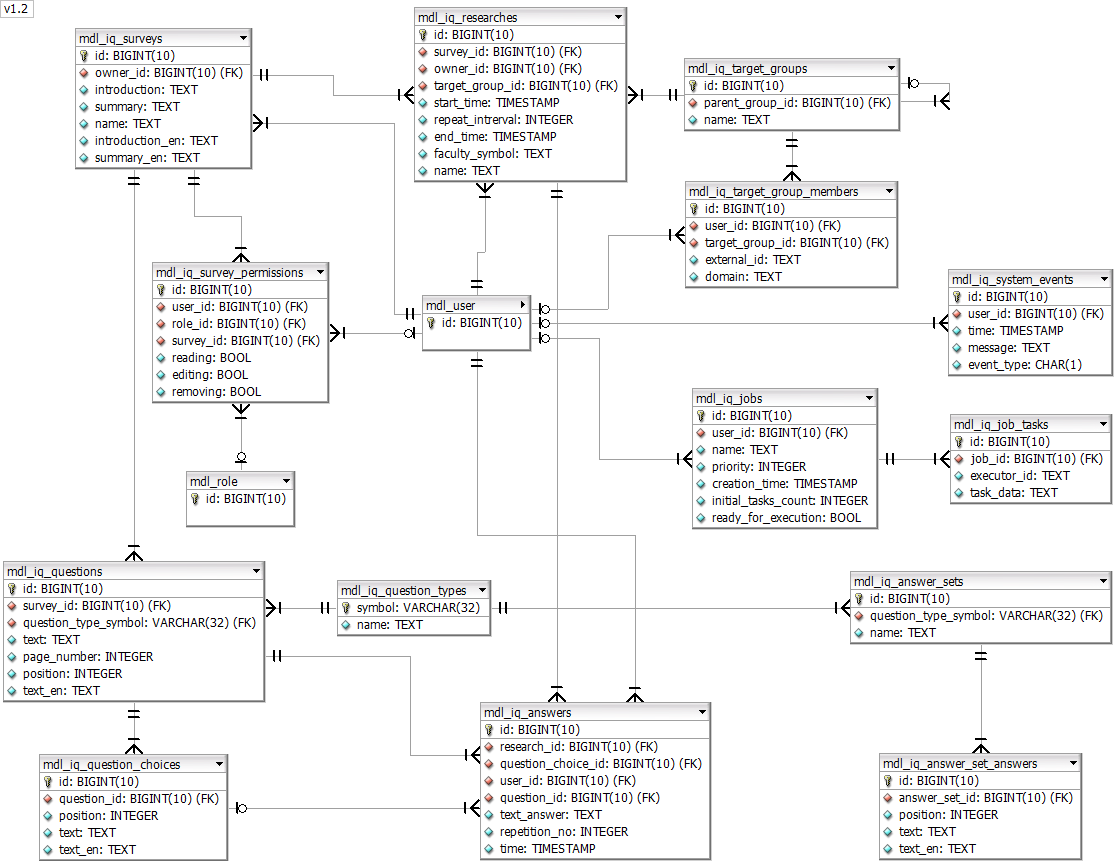
\includegraphics[height=\textheight, width=1.5\textwidth]{figures/iQuest_Database}
\caption{Diagram Bazy Danych}\label{rys:iQuest_DataBase}
\end{figure}
\end{landscape}
\chapter{Opis implementacji}
\label{Chapter6}

\section{Wstęp}
\label{Chapter61}

{\color{red}Wersja bez redakcji.}

%Wprowadzenie. Struktura tego rozdziału nie jest z góry określona, gdyż mocno zależy to od specyfiki projektu. Generalnie w poszczególnych podrozdziałach każdy powinien opisać swoją część z takiego technicznego punktu widzenia. Piszecie, jak zrealizowaliście poszczególne wymagania, jak to wygląda ,,pod maską'', oczywiście też trzeba przyjąć jakiś poziom szczegółowości. W bardzo szczególnych przypadkach chyba może się zdarzyć, że trzeba będzie załączyć fragment jakiegoś kodu źródłowego czy konfiguracji -- generalnie ma to być opisane w taki sposób, że jako osoba nieznająca systemu siadam i wiem, jak i co zrobiliście. Oczywiście, to moje dywagacje, być może osoby związane z uczelnią zlinczują mnie za ten fragment.

\section{Napotkane problemy i ich rozwiązania}
\label{Chapter62}
%Tu zostanie przeniesiona część treści z wniosków. Wówczas dodane zostaną odpowiednie lub zastosowany zostanie ten sam mechanizm co we Wnioskach.

\section{Użyte technologie}
\label{Chapter63}

\subsection{Moodle}
\emph{Moodle} (roz. \textit{Modular Object-Oriented Dynamic Learning Environment}) -- stanowi podstawę systemu \textit{iQuest}. Jest to popularna (ponad 63 miliony użytkownikiów) platforma e-learningowa o otwartym kodzie źródłowym, napisana w języku \emph{PHP}.Wyboru dokonano ze względu na kilka czynników:
\begin{itemize}
\item{Propozycję Architekta, wynikającą z faktu, iż Moodle posiada już implementację wielu wymaganych w \textit{iQuest} mechanizmów, jak np. konta użytkowników, system ról i uprawnień.}
\item{Oczekiwania Klienta, wynikające z popularności platformy Moodle wśród systemów uczelnianych.}
\item{Modułowość \emph{Moodle}, umożliwiającą pisanie rozszerzeń.}
\end{itemize}

\subsection{PHP}
\emph{PHP} -- platforma \textit{Moodle} jest napisana właśnie w tym języku programowania. Z tego względu, jest to technologia zastosowana w większości rozszerzeń utworzonych przez zespół /textit{iQuest}, korzystających z interfejsów programowania aplikacji tej platformy. Ponadto \emph{PHP} jest jednym z najpopularniejszych języków programowania aplikacji internetowych, posiada doskonalą dokumentację oraz jest cały czas rozwijany.

\subsection{PHPUnit}
Ze względu na fakt, iż programiści \textit{Moodle'a} wykonują testy jednostkowe kodu wykorzystując do tego celu \emph{PHPUnit}, zdecydowano się skorzystać z przygotowanego przez nich oprogramowania. \textit{Moodle} udostępnia dwie klasy do testowania -- \textit{basic\_testcase} i \textit{advanced\_testcase}, przy czym druga wymieniona służy do testów, które wchodzą w interakcję z bazą danych.

\subsection{Selenium}
\emph{Selenium} -- szybko rozwijające się narzędzie do testów akceptacyjnych. Był to naturalny wybór zwłaszcza, że zostało ono przybliżone programistom na zajęciach z Inżynierii Oprogramowania w trakcie toku studiów. Projekt ten składa się m.in. z następującego oprogramowania:
\begin{itemize}
\item{Selenium IDE -- zintegrowane środowisko programistyczne dla skryptów \emph{Selenium} -- zaimplementowane jako rozszerzenie dla przeglądarki internetowej Firefox. Pozwala na: nagrywanie i odtwarzanie sekwencji kroków, wykonywanych podczas pracy z przeglądarką, eksport skryptów do kodu języków programowania (np. \emph{Java}).}
\item{Selenium Client Drivers (\emph{Java}) -- sterownik klienta dla języka Java, pozwalający na wykonywanie skryptów \emph{Selenium} z poziomu języka \emph{Java}},
\item{HtmlUnit Driver} -- Implementacja klasy \emph{WebDriver}, która emuluje zachowanie przeglądarki. Pozwala na uruchamianie skryptów \emph{Selenium} bez korzystania z przeglądarki internetowej.}
\end{itemize}

\subsection{PostgreSQL}
System zarządzania bazą danych \emph{PostgreSQL} został wybrany ze względu na wymaganie pozafunkcjonalne -- pracownicy \emph{Działu Rozwoju Oprogramowania Politechniki Poznańskiej} korzystają z tej właśnie bazy danych. Jest to baza danych o otwartym kodzie źródłowym, zgodna ze standardami, ciągle rozwijana, wysoce konfigurowalna.

\subsection{Eclipse IDE}
\label{Chapter621}

Wybór \emph{Eclipse IDE} jako stosowanego dla projektu \textit{iQuest} zintegrowanego środowiska programistycznego wynika z faktu, iż oprogramowanie to jest dostępne za darmo. Dodatkową zaletą \textit{Eclipse} jest modularność tego rozwiązania, dzięki czemu dostępny jest w nim dodatek \emph{PHP Development Tools}, upraszczający pracę z technologią PHP. Udostępnia m.in. narzędzia do analizy poprawności składniowej pisanego kodu, formatery kodu, wyszukiwanie fraz w wielu plikach, kontekstowe podpowiedzi i nawigację.

\subsection{SVN}
\label{Chapter632}

\emph{Subversion} został wybrany jako podstawowy system kontroli wersji ze względu na wymagania pozafunkcjonalne. Zespół eksploatacji, który docelowo przejmie zarządzanie artefaktami związanymi z projektem, wykorzystuje właśnie \textit{SVN}. Główne funkcjonalności tego systemu to: atomowe publikowanie zmian, historia operacji na plikach (zmiana nazwy, skopiowanie, przeniesienie, modyfikacja, usunięcie), wersjonowanie plików i folderów, łatwy dostęp do informacji o zmianach.

\subsection{Redmine}
\label{Chapter633}

Systemu zarządzania projektami \emph{Redmine} wykorzystywany był od samego początku istnienia projektu. Jest to narzędzie bardzo przydatne w wymianie informacji pomiędzy członkami zespołu, integrujące się m.in. z repozytorium kodu, bazą wiedzy o projekcie, listą zagadnień, forum.  Technologia ta została narzucona, ze względu na sposób organizacji pracy w \textit{Software Development Studio} na Politechnice Poznańskiej.

\subsection{JasperReports}
\label{Chapter634}

Ze względu na wymagania pozafunkcjonalne, zdecydowano się skorzystać z mechanizmów raportowania oferowanych przez \emph{JasperReports}. Jest to najbardziej popularny silnik raportowania o otwartym kodzie źródłowym (wersja Community). Pozwala na generację raportów, których treść jest określona z dokładnością co do piksela. Generowane raporty można eksportować do popularnych formatów dokumentów, np. HTML, PDF, Excel, Word.
\subsection{\textit{JavaScript}}
\label{Chapter63b}

Formularze wymagające częstej interakcji z klientem, np. formularz umożliwiający tworzenie nowej ankiety, oraz funkcje związane z walidacją pól uzupełnianych przez klienta zostały napisane w \textit{JavaScript}. Obsługa strony po stronie klienta jest dla użytkownika niego znacznie wygodniejsza, gdyż nie wymaga częstego przeładowywania całej strony. Dodatkowo, ogranicza to obciążenie łącza zarówno po jego stronie, jak i po stronie serwera, co jest korzystne dla obu stron.

\section{Ogólna struktura projektu}
\label{Chapter64}

{\color{red}Sekcja druga.}

\section{Interfejs}
\label{Chapter65}

Jedną z części pracy było zaprojektowanie graficznego interfejsu użytkownika. Głównym problemem jaki się pojawił, był wybór odpowiedniego narzędzia. Celem jaki postawiono, była maksymalna zgodność projektowanych elementów z różnymi wersjami \emph{Moodle} -- zarówno wcześniejszymi, jak i późniejszymi. Zdecydowano, aby starać się korzystać z gotowych interfejsów programowania aplikacji \emph{(API)} dostarczonych przez \emph{Moodle}, tj. \emph{Page API}, \emph{Form API}, oraz \emph{Access API}. Wszystkie interfejsy są napisane przy użyciu języka PHP -- są wykonywane po stronie serwera. Konieczne okazało się też wykonanie niektórych skryptów po stronie klienta. Dlatego w projekcie wykorzystano również język skryptowy \emph{Java Script}.

\section{Logika (back-end)}
\label{Chapter66}

Jednym z zadań w ramach pracy było zaprogramowanie odpowiedniej logiki biznesowej rozwiązującej zadania stawiane przed zaprojektowanym systemem. Najważniejszym zadaniem z perspektywy back-end'u jest interakcja z bazą danych. Poza tym system posiada: procesor zadań wykonywanych w tle oparty na \emph{cron}; moduły odpowiadające za komunikację z systemami uczelanianymi \emph{ePoczta} i \emph{eDziekanat}; moduł logowania zdarzeń. W trakcie implementacji zdecydowano się nie tworzyć osobnego mechanizmu do przechowywania ustawień w bazie danych i skorzystaliśmy z istniejącego już w \emph{Moodle}. Jednym z wymagań pozafunkcjonalnych było wykorzystanie bazy danych \emph{PostgreSQL}. Platforma \emph{Moodle} korzysta z mechanizmu \emph{XMLDB}, co pozwala na ominięcie wielu problemów pojawiających się przy migracjach pomiędzy różnymi systemami baz danych. Niestety kosztem wykorzystania tego mechanizmu jest konieczność pracy z interfejsami programowania aplikacji dostarczanym przez platformę \emph{Moodle} -- \emph{Data manipulation API}. Na diagramie poniżej znajdują się także klasy przechowujące stałe: (\emph{tables}, \emph{settings}.\\

\begin{figure}[H]
\begin{center}
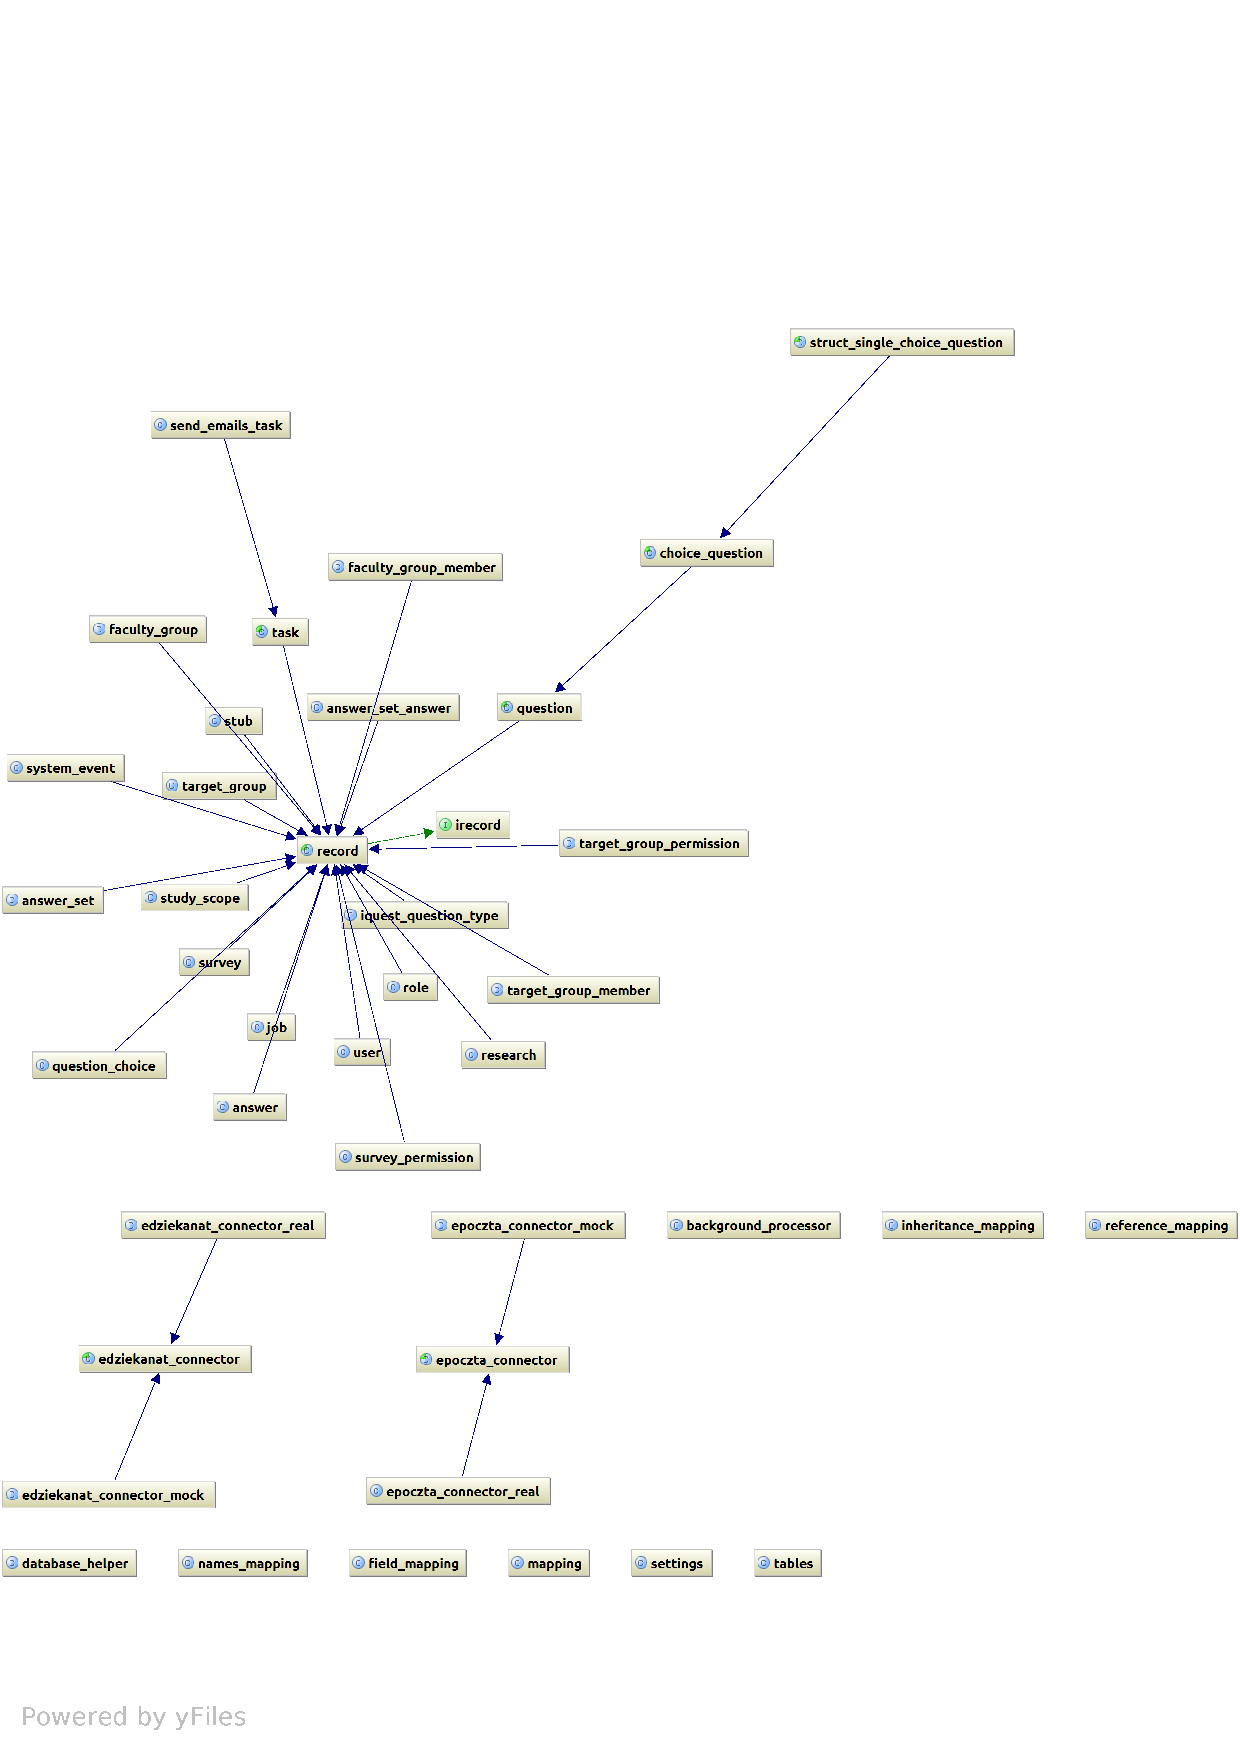
\includegraphics[width=0.9\textwidth]{figures/lw/backend.pdf} 
\end{center}
\caption{Struktura back-end'u}
\label{fig:back-end}
\end{figure}

\subsection{Raporty}
Raporty wykonano korzystając z platformy JasperReports, wykorzystując następujące produkty firmy \emph{Jaspersoft}:

\begin{itemize}
\item \emph{JasperReports Server} (wersja 5.0) -- serwer usług raportowania, na którym przechowywane są przygotowane przez zespół artefakty, w celu umożliwienia generacji raportu osobom dysponującym odpowiednimi uprawnieniami. Wykorzystano następujące funkcjonalności: definiowania źródła danych, raportu, ładowania plików z projektem raportu, zasobami oraz z generacji raportu.
\item \emph{Jaspersoft Studio} (wersja 1.3.2) -- bazowane na Eclipse narzędzie do projektowania raportów. Posłużyło zespołowi do przygotowania projektów raportów w formacie \emph{JRXML}.
\end{itemize}

Kody źródłowe pakietu \emph{JasperReports} są pisane w języku Java. Źródłem danych dla raportu, jest przygotowana przez zespół implementacja interfejsu \emph{ReportDataSourceService} z \emph{API JasperServer}. Źródło danych łączy się z udostępnianymi przez wskazaną instancję systemu \emph{iQuest} usługami zdalnymi, z których otrzymuje informacje o przeprowadzanych badaniach poprzez protokół SOAP. Struktura raportu zależy od typu pytania (otwarte/zamknięte). W przypadku pytań otwartych prezentowana jest lista odpowiedzi. Dla pytań zamkniętych na podstawie pobranych danych generowane są statystyki, które przekazywane są do podraportu w postaci obiektu klasy \emph{JRBeanCollectionDataSource}. W generacji statystyk z danych badań wykorzystano bibliotekę \emph{JoSQL}. Definicja projektu raportu składa się z czterech plików, odpowiadających trzem kolejnych poziomom:
\begin{enumerate}
\item \emph{researches.jrxml} -- raport główny dla badań,
\item \emph{questions.jrxml} -- podraport pytań,
\item \emph{answers\_closed.jrxml} oraz \emph{answers\_open.jrxml} -- podraporty odpowiedzi. zamkniętych i otwartych.
\end{enumerate}
Do generacji namiastek obiektów zdalnych (ang. \definicja{stub}) wykorzystano Apache Axis. Wygenerowane klasy dostosowano tak, by akceptowały obiekty z zadanej instancji \emph{iQuest} oraz dla zmiennej przestrzeni nazw (ang. \emph{namespace}).\\

W trakcie generacji \emph{stub'ów} okazało się, iż definicja usług dla protokołu \emph{SOAP} w języku \emph{WSDL} (\emph{Web Service Description Language}) generowana przez \emph{Moodle} jest niepoprawna. Skorzystano zatem z poprawionej wersji z zewnętrznego źródła (\url{https://github.com/ghigio/moodle-webservice_soapfda}).\\

Dostęp do usług zdalnych definiowanych w \emph{Moodle} zabezpieczono korzystając z mechanizmu generacji tokenu dla wybranego użytkownika. Użytkownik, który z poziomu serwera \emph{Jasper Server} zamierza wygenerować raport, musi znać adres naszego systemu oraz posiadać token dostępu do usługi.

\subsection{Moduły uwierzytelniania}
Korzystając z mechanizmów rozszerzeń \emph{Moodle} zaimplementowano dwa moduły uwierzytelniania, tj.:
\begin{itemize}
\item \emph{eKontoAuthenticationPlugin} -- integruje logowanie przez \emph{eKonto} z naszym systemem,
\item \emph{emailgraduate} -- pozwala absolwentom uczelni na rejestrację z użyciem adresu e-mail.
\end{itemize}

W celu spełnienia wymagań Działu Rozwoju Oprogramowania Politechniki Poznańskiej odnośnie wygaszania sesji użytkownika \emph{eKonto} po zadanym czasie (e.g. 15 min.) zmodyfikowano pliki źródłowe \emph{Moodle}, gdyż dla kodu odnoszącego się do sesji użytkownika \emph{Moodle} nie została przewidziana możliwość rejestracji rozszerzeń. Relacja \emph{user} została rozszerzona o opcjonalne pola związane z \emph{eKonto}, jako że kod odpowiedzialny za manipulację schematem bazy danych nie jest wykonywany podczas instalacji modułu uwierzytelniania, umieszczono go w osobnym module (\emph{ekontodb}). \emph{eKontoAuthenticationPlugin} może być instalowany bez konieczności instalacji \emph{iSurvey}. Podczas jego implementacji korzystaliśmy z dokumentu \emph{Centralne uwierzytelnianie i wymiana danych. Wersja 1.2 (2010.07.06)}.\\

Podczas rejestracji z użyciem naszych modułów użytkownik jest przydzielany do grupy docelowej ,,Absolwenci'', nadawana jest mu też rola respondenta w kontekście \emph{kursu iQuest}. Utworzenie modułu wiąże się z przygotowaniem klasy dziedziczącej z \emph{auth\_plugin\_base}, formularza ustawień, pliku lokalizacji oraz wersji.

\subsection{Moduły dla serwisów zewnętrznych}
\begin{itemize}
\item \emph{ePocztaConnector} -- służy do wysyłania e-maili z serwera Politechniki Poznańskiej,
\item \emph{eDziekanatConnector} -- pobiera i aktualizuje lokalne informacje o grupach dziekańskich, zakresach tematycznych tychże grup oraz ich studentach.
\end{itemize}

\emph{Dział Rozwoju Oprogramowania} udostępnia klienty \emph{eUsług} dla różnych języków, w tym dla \emph{PHP}. Komunikacja z usługami zdalnymi uczelni odbywa się poprzez protokół SOAP. Wyżej wymienione moduły zaimplementowano z wykorzystaniem fabryki obiektów, która w zależności od trybu (testowy/produkcyjny) zwraca obiekt odpowiedniej klasy. Zadania związane z oba modułami są zlecane procesorowi zadań w tle.

%to poleci gdzieś indziej.
%\begin{landscape}

%\begin{figure}[!th]
%\centering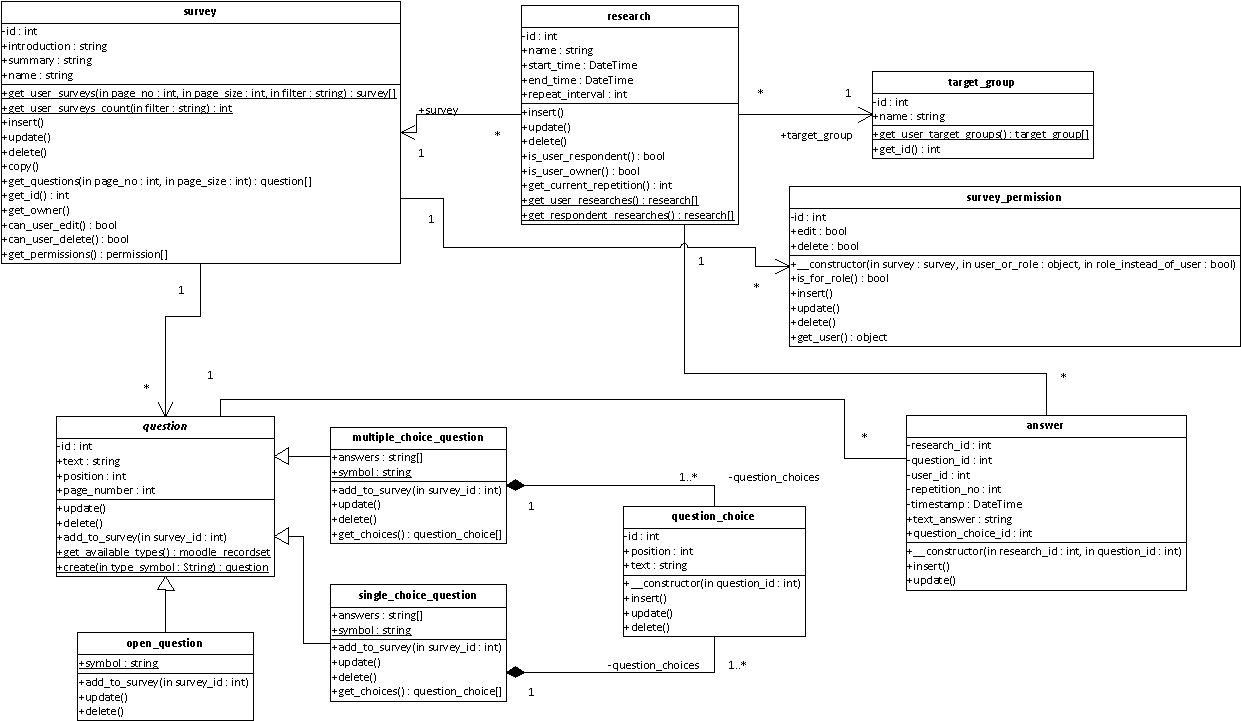
\includegraphics[width=1.25\textheight]{figures/Survey_Creator_Survey_Runner.png}
%\caption{Backend -- moduły Survey Creator i Survey Runner}\label{rys:iquest-backend}
%\end{figure}

%\begin{figure}[!th]
%\centering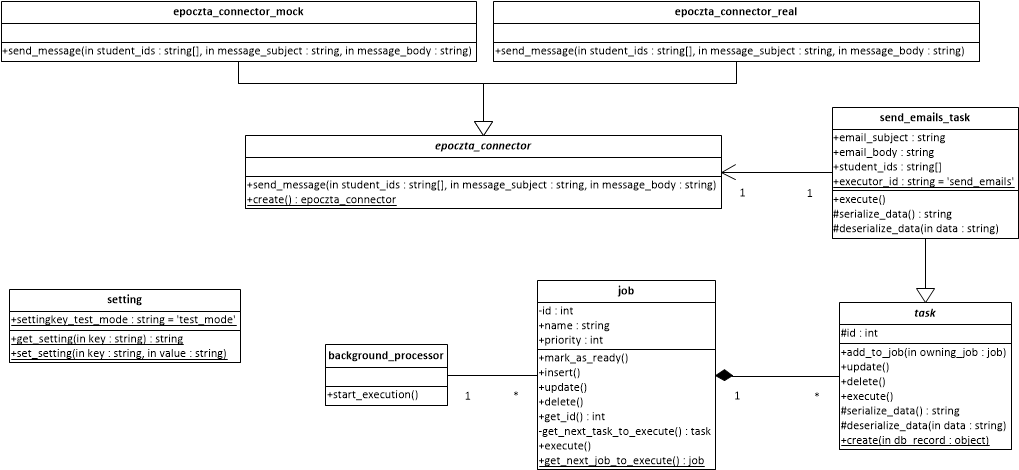
\includegraphics[width=1.25\textheight]{figures/ePoczta_Connector_Background_Task_Scheduler_and_Executor.png}
%\caption{Backend -- moduły ePoczta Connector i Background Task Scheduler and Executor}\label{rys:iquest-backend2}
%\end{figure}

%\end{landscape}

\section{Powiązanie back-endu z interfejsem}
\label{Chapter67}

%brak treści?
\chapter{Zapewnianie jakości i konserwacja systemu}
\label{Chapter7}

\section{Testy i weryfikacja jakości oprogramowania}
\label{Chapter71}

\subsection{Wstęp}
\label{Chapter711}

Testy i weryfikacja jakości oprogramowania realizowana była na trzech poziomach: testów jednostkowych (dla logiki) oraz automatycznych i manualnych testów akceptacyjnych. Te ostatnie realizowane były nie tylko w zgodzie z dokumentem \textit{MAT}\cite{Redmine:ProjDocs}, ale też intuicyjnie, poprzez zwykłe korzystanie z systemu.

\subsection{Testy jednostkowe}
\label{Chapter712}

Testy jednostkowe zostały wykonane jako pierwsze i traktowane były z wysokim priorytetem. Realizowane były z użyciem klas PHPUnit, stosowanych powszechnie m.in.~przy testowaniu wtyczek do platformy Moodle. Testy te były kluczowe dla rozwoju logiki systemu iQuest. Przygotowaliśmy konfigurowalne skrypty automatyzujące proces testowania w języku BASH. Część testów operuje na systemie w trybie produkcyjnym, część na trybie testowym, obsługującym tzw. ,,atrapy'' (ang. \definicja{mock}), imitujące działanie systemów zewnętrznych poprzez zwracanie przykładowych danych.\\

Przy realizacji pierwszego wydania, za testy jednostkowe w pełni odpowiadał jeden z członków zespołu programistów. W wydaniu drugim, rolę tę przejął programista realizujący logikę systemu. Z początku próbowaliśmy działać w oparciu o TDU (ang. \definicja{Test-Driven Development} - rozwój w oparciu o testy), jednakże szybko porzuciliśmy tą metodykę, ze względu na brak doświadczenia programistów.

Na początku projektu przygotowaliśmy program w języku Java uruchamiający zestaw testów akceptacyjnych. W drugim wydaniu korzystaliśmy już wyłącznie z Selenium IDE, ze względu możliwość szybszego rozpoznania problemów z poziomu przeglądarki, w przeciwieństwie do terminala.

\newpage
\begin{figure}[H]
\begin{center}
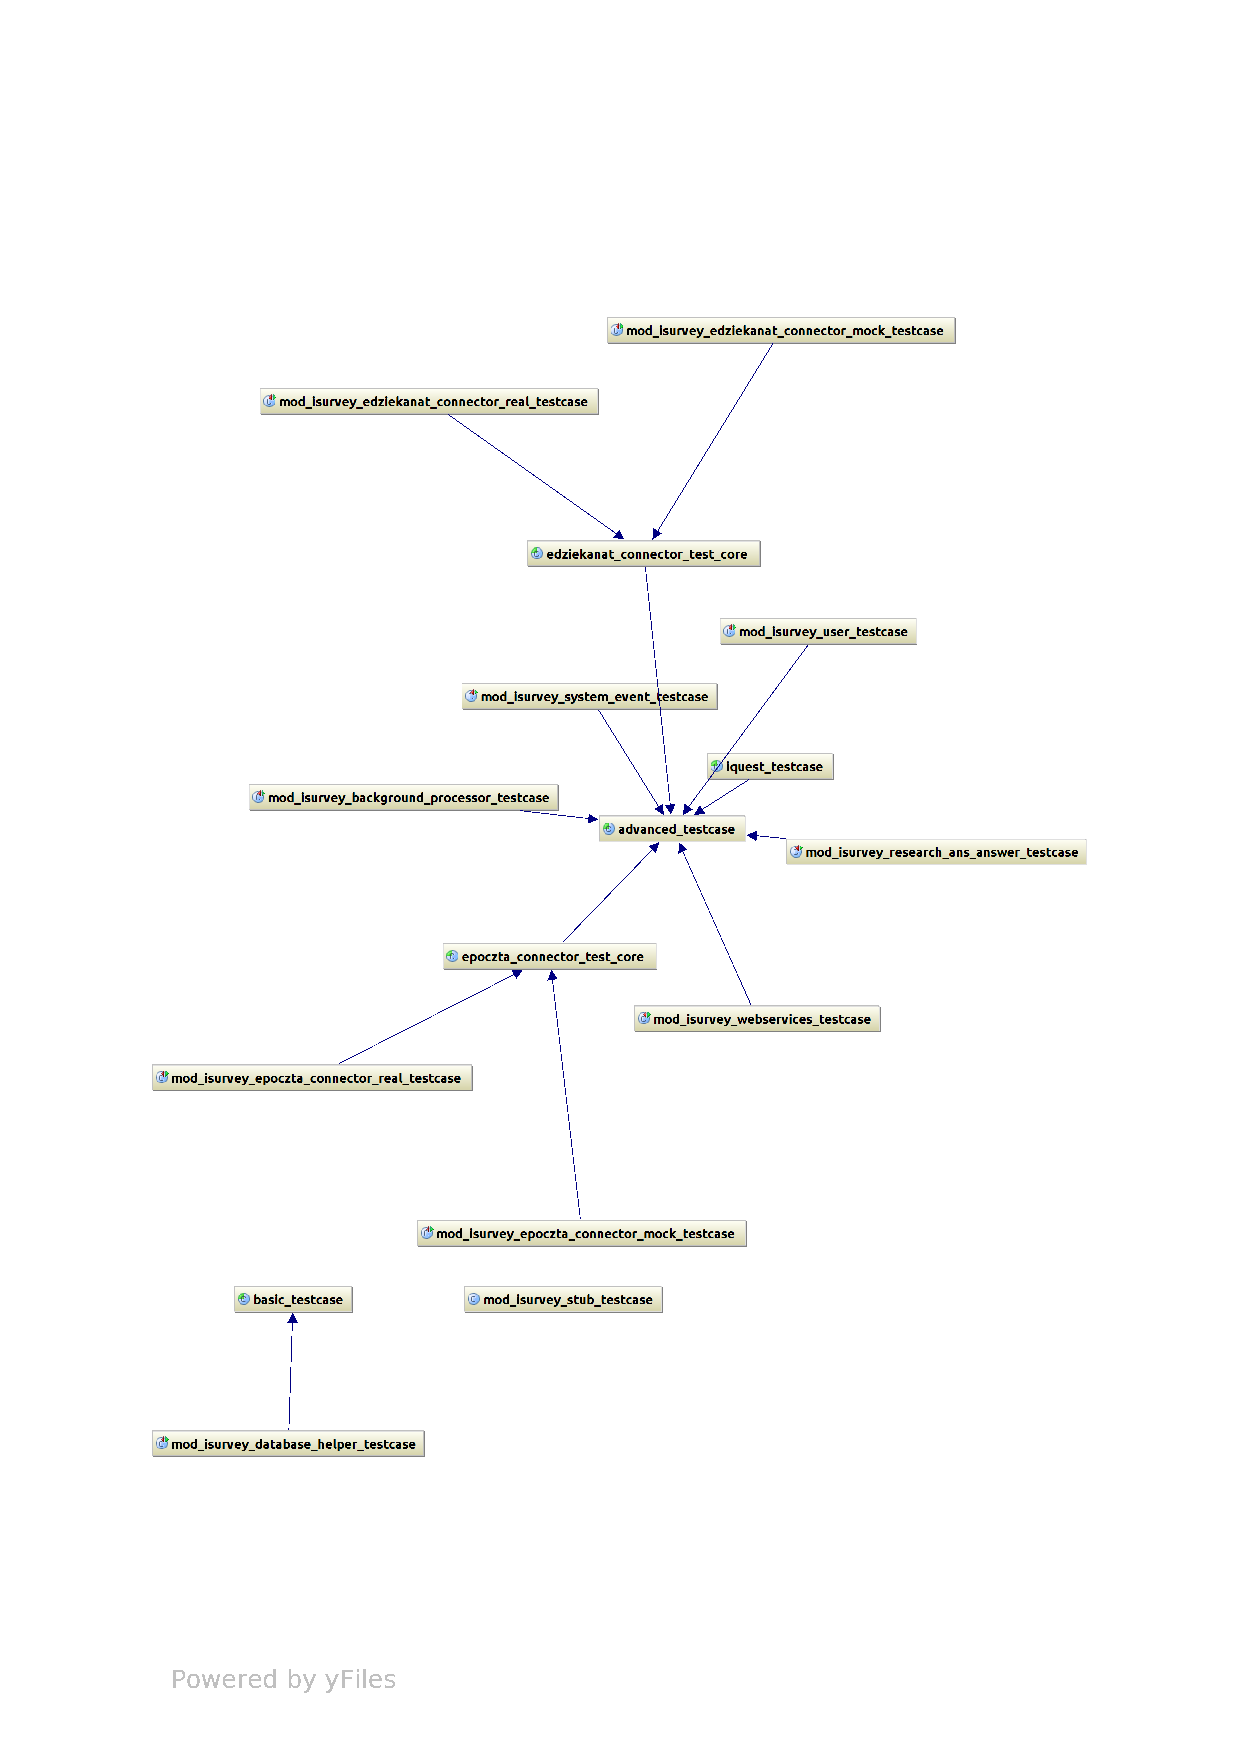
\includepdf{figures/lw/tests1.pdf} 
\end{center}
\caption{Struktura klas testujących (1)}
\label{fig:tests1}
\end{figure}
\newpage
\begin{figure}[H]
\begin{center}
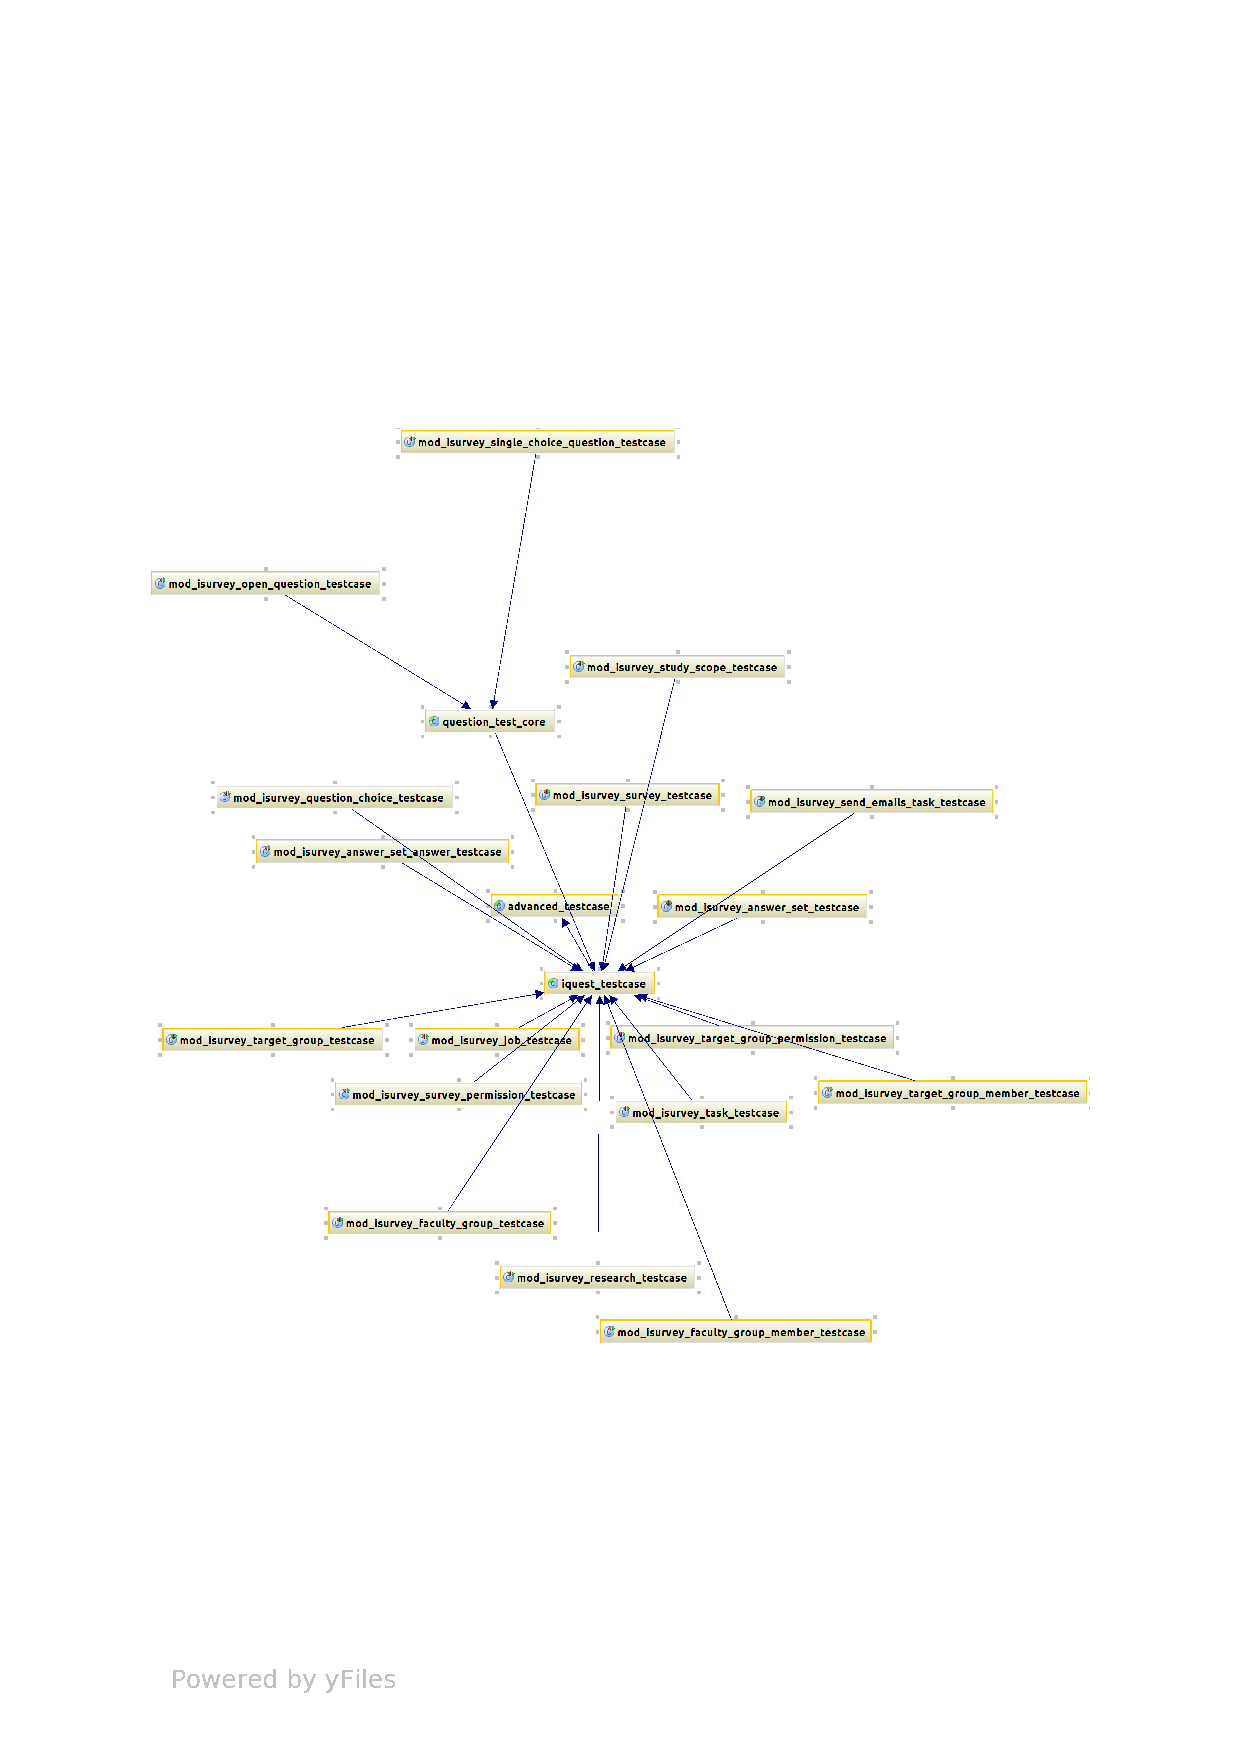
\includepdf{figures/lw/tests2.pdf} 
\end{center}
\caption{Struktura klas testujących (2)}
\label{fig:tests2}
\end{figure}
\newpage

Na diagramach widzimy trzy klasy służące do testowania, z których dziedziczą wszystkie inne, są to:
\begin{itemize}
\item \emph{basic\_testcase} -- podstawowe testy jednostkowe
\item \emph{advanced\_testcase} -- testy z użyciem bazy danych
\item \emph{iquest\_testcase} -- rozszerzenie \emph{advanced\_testcase} na potrzeby testowania klas dziedziczących z \emph{record}
\end{itemize}

\subsection{Testy akceptacyjne}
\label{Chapter713}

Testy akceptacyjne rozpatrywane są na dwóch poziomach: automatycznym i manualnym. Różnica polega jedynie na tym, kto (lub co) wykonuje test - komputer z odpowiednim oprogramowaniem, czy człowiek.

\subsubsection{MAT}
\label{Chapter7131}
{\color{red}Testy akceptacyjne wymagają poprawienia -- dane od zespołu zarządzającego były nieaktualne!!!}
Poniżej przedstawiono Manualne Testy Akceptacyjne:

\matbegin{TC1}{Logowanie do systemu przez eKonto}
\matpres
\matpre{Użytkownik jest niezalogowany}
\matpre{Użytkownik posiada eKonto}
\matpre{Połączenie z Internetem}
\matsteps
\matstep{1}{Użytkownik wpisuje adres systemu}{Strona logowania do system iQuest}
\matstep{2}{Użytkownik naciska przycisk ,,Zaloguj przez eKonto''}{Strona logowania eLogin}
\matstep{3}{Użytkownik wpisuje dane logowania}{}
\matstep{4}{Użytkownik naciska przycisk ,,Zaloguj''}{Przekierowanie na stronę systemu iQuest, wyświetlenie strony głównej z zalogowanym użytkownikiem.}
\matremark{}

\matbegin{TC2}{Stworzenie Ankiety}
\matpres
\matpre{Zalogowany użytkownik z prawem do tworzenia ankiet}
\matsteps
\matstep{1}{Użytkownik wybiera przycisk ,,Stwórz ankietę''}{Strona umożliwiająca tworzenie ankiet}
\matstep{2}{Użytkownik podaje nazwę ankiety}{}
\matstep{3}{Użytkownik podaje wstęp  i podsumowanie ankiety}{}
\matstep{4}{Użytkownik dodaje pytanie jednokrotnego wyboru}{Pojawia się pole na wpisanie treści pytania}
\matstep{5}{Użytkownik wpisuje treść pytania}{}
\matstep{6}{Użytkownik naciska przycisk „Dodaj odpowiedź'' dwukrotnie}{Pojawiają się dwa pola do wpisania możliwych odpowiedzi}
\matstep{7}{Użytkownik podaje treści możliwych odpowiedzi}{}
\matstep{8}{Użytkownik dodaje stronę wciskając przycisk „Dodaj stronę''}{Wyświetla się nowa strona na dodawanie pytań}
\matstep{9}{Użytkownik dodaje pytanie otwarte}{Wyświetla się pole na wpisanie treści pytania}
\matstep{10}{Użytkownik wpisuje treść pytania}{}
\matstep{11}{Użytkownik wybiera przycisk „Zapisz zmiany''}{Komunikat o pomyślnym stworzeniu ankiety}
\matremark{}

\begin{table}[H]
\centering
\begin{tabular}{ | >{\bfseries}c | p{5cm} | } \hline
Krok & \textbf{Dane} \\ \hline
2 & ,,Ankieta testowa'' \\ \hline
3 & ,,Wstęp'' oraz ,,Podsumowanie'' \\ \hline
5 & ,,Pytania jednokrotnego wyboru działają?'' \\ \hline
7 & ,,tak'' oraz ,,nie'' \\ \hline
10 & ,,Pytania otwarte działają?'' \\ \hline
\end{tabular}
\caption{Poprawne dane dla scenariusza TC2}\label{tab:TC2-correct}
\end{table}

\matbegin{TC2.2}{Stworzenie Ankiety - brak pytań}
\matpres
\matpre{Zalogowany użytkownik z prawem do tworzenia ankiet}
\matsteps
\matstep{1}{Użytkownik wybiera przycisk „Stwórz ankietę''}{Strona umożliwiająca tworzenie ankiet}
\matstep{2}{Użytkownik podaje nazwę ankiety}{}
\matstep{3}{Użytkownik podaje wstęp  i podsumowanie ankiety}{}
\matstep{4}{Użytkownik wybiera przycisk „Zapisz zmiany''}{Komunikat o braku pytań w ankiecie}
\matremark{}

\matbegin{TC3}{Edycja ankiety}
\matpres
\matpre{Zalogowany użytkownik z prawem do tworzenia ankiet}
\matpre{Użytkownik posiada prawo do edycji ankiety ,,Ankiety testowej''}
\matsteps
\matstep{1}{Użytkownik wybiera przycisk „Katalog Ankiet''}{Strona z listą ankiet do których prawo ma użytkownik.}
\matstep{2}{Użytkownik wybiera przycisk „edytuj'' przy „Ankiecie Testowej''}{Strona umożliwiająca edycję „Ankiety Testowej''}
\matstep{3}{Użytkownik wciska przycisk „usuń'' przy pytaniu drugim}{Pytanie drugie znika}
\matstep{4}{Użytkownik naciska przycisk „Dodaj odpowiedź'' przy pytaniu pierwszym}{Pojawia się pole do wpisania możliwej odpowiedzi}
\matstep{5}{Użytkownik wpisuje możliwą odpowiedź}{}
\matstep{6}{Użytkownik wybiera przycisk „Zapisz zmiany''}{Strona wyświetla komunikat potwierdzający zapisanie zmian w ankiecie.}
\matremark{}

\begin{table}[H]
\centering
\begin{tabular}{ | >{\bfseries}c | p{5cm} | } \hline
Krok & \textbf{Dane} \\ \hline
5 & ,,nie wiem'' \\ \hline
\end{tabular}
\caption{Poprawne dane dla scenariusza TC3}\label{tab:TC3-correct}
\end{table}

\matbegin{TC3}{Edycja ankiety - usunięcie wszystkich pytań}
\matpres
\matpre{Zalogowany użytkownik z prawem do tworzenia ankiet}
\matpre{Użytkownik posiada prawo do edycji ankiety ,,Ankiety testowej''}
\matsteps
\matstep{1}{Użytkownik wybiera przycisk „Katalog Ankiet''}{Strona z listą ankiet do których prawo ma użytkownik.}
\matstep{2}{Użytkownik wybiera przycisk „edytuj'' przy „Ankiecie Testowej''}{Strona umożliwiająca edycję „Ankiety Testowej''}
\matstep{3}{Użytkownik wciska przycisk „usuń'' przy każdym z pytań}{Pytania znikają}
\matstep{4}{Użytkownik wybiera przycisk „Zapisz zmiany''}{Strona wyświetla komunikat, że ankieta nie posiada pytań i prosi o ich dodanie.}
\matremark{}

\matbegin{TC4}{Wybranie grupy docelowej}
\matpres
\matpre{Zalogowany użytkownik z prawami do tworzenia ankiet}
\matpre{Użytkownik posiada prawa do ankiety „Ankieta Testowa''}
\matpre{Użytkownik posiada prawo do ankietowania grupy docelowej „test''}
\matsteps
\matstep{1}{Użytkownik wybiera przycisk ,,Włącz tryb edycji''}{Interfejs edycji Moodle}
\matstep{2}{Użytkownik wybiera przycisk „edytuj'' przy „Ankiecie Testowej''}{Strona umożliwiająca edycję „Ankiety Testowej''}
\matstep{3}{Użytkownik wybiera grupę docelową „test''}{}
\matstep{4}{Użytkownik wybiera przycisk „Zapisz zmiany''}{Strona wyświetla komunikat, że ankieta została zaktualizowana pomyślnie.}
\matstep{5}{Respondent otrzymuje email z powiadomieniem o ankiecie}{}
\matremark{}

\matbegin{TC5}{Udzielanie odpowiedzi}
\matpres
\matpre{Zalogowany użytkownik}
\matpre{Użytkownik znajduje się w grupie docelowej ankiety ,,testowa''}
\matpre{Użytkownik nie odpowiadał udzielał odpowiedzi na ankietę ,,testowa''}
\matsteps
\matstep{1}{System prezentuje ankiety na które użytkownik jeszcze nie odpowiedział}{}
\matstep{2}{Użytkownik wybiera ankietę ,,testowa''}{System prezentuje ankietę}
\matstep{3}{Użytkownik zaznacza odpowiedź na pytanie 1 jako ,,tak''}{}
\matstep{4}{Użytkownik podaje odpowiedź na pytanie drugie jako ,,tak''}{}
\matstep{5}{Użytkownik potwierdza wypełnienie ankiety przyciskiem ,,Wyślij''}{System prezentuje ankiety na które użytkownik jeszcze nie odpowiedział oraz komunikat o pomyślnym przesłaniu odpowiedzi}
\matstep{6}{Respondent otrzymuje email z powiadomieniem o ankiecie}{}
\matremark{}

\matbegin{TC6}{Sprawdzenie wyników}
\matpres
\matpre{Zalogowany użytkownik z prawem do oglądania wyników ankiety ,,Testowa''}
\matsteps
\matstep{1}{Użytkownik wybiera badanie, którego podstawowe wyniki chce sprawdzić}{System prezentuje podsumowanie ankiety}
\matremark{Dotyczy podstawowych wyników. Wyniki zaawansowane obsługuje zewnętrzny serwer BI}

\matbegin{TC7}{Dodawanie grupy docelowej}
\matpres
\matpre{Zalogowany administrator z prawami do tworzenia grup docelowych}
\matpre{Brak w systemie grupy docelowej ,,Grupa 1''}
\matsteps
\matstep{1}{Administrator wybiera przycisk ,,Zarządzaj grupami docelowymi''}{System prezentuje dostępne grupy docelowe w systemie}
\matstep{2}{Administrator wybiera przycisk ,,dodaj''}{System prezentuje interfejs dodawania grupy docelowej}
\matstep{3}{Administrator podaję nazwę nowej grupy „Grupa 1” i wskazuje jej członków}{}
\matstep{4}{Administrator wybiera grupę nadrzędną dla nowej grupy docelowej}{System automatycznie zapisują zmiany}
\matremark{Test przygotowany na podstawie makiety systemu iQuest}

\matbegin{TC8}{Edycja grupy docelowej}
\matpres
\matpre{Zalogowany administrator z prawami do tworzenia grup docelowych}
\matpre{Grupa docelowa ,,Grupa 1'' istnieje w systemie}
\matsteps
\matstep{1}{Administrator wybiera przycisk ,,Zarządzaj grupami docelowymi''}{System prezentuje dostępne grupy docelowe w systemie}
\matstep{2}{Administrator wybiera przycisk ,,zmień nazwę''}{System prezentuje interfejs zmiany nazwy grupy docelowej}
\matstep{3}{Administrator pozostawia nazwę niezmienioną i zatwierdza zmiany}{System prezentuje dostępne grupy docelowe w systemie}
\matstep{4}{Administrator wybiera grupę nadrzędną dla grupy docelowej i dodaje nowego członka do grupy}{System automatycznie zapisują zmiany}
\matremark{Test przygotowany na podstawie makiety systemu iQuest}

\matbegin{TC9}{Edycja grupy docelowej}
\matpres
\matpre{Użytkownik jest niezalogowany}
\matpre{Istnieje konto użytkownika w systemie}
\matsteps
\matstep{1}{Użytkownik wpisuje adres systemu}{Strona główna moodla z kursem iQuest}
\matstep{2}{Użytkownik naciska przycisk ,,Zaloguj się''}{Strona logowania}
\matstep{3}{Użytkownik wpisuje dane logowania}{}
\matstep{4}{Użytkownik naciska przycisk ,,Zaloguj się''}{Przekierowanie na główną stronę moodla z kursem iQuest. Wyświetla się napis: ,,Jesteś zalogowany(a) jako...''}
\matremark{}

{\color{red}Niedodane jeszcze TC: Logowanie bez eKonta, }

Dodatkowo, poniżej znajduje się wykaz mapujący przypadki testowe do przypadków użycia:
\begin{itemize}
\item{TC1.X – UC09 Logowanie do systemu.}
\item{TC2.X – UC01 Stworzenie ankiety}
\item{TC3.X – UC02 Edycja ankiety}
\item{TC4.X – UC03 UC04 Wybranie grupy docelowej, uruchomienie ankiety}
\item{TC5.X – UC05 Udzielenie odpowiedzi}
\item{TC6.X – UC06 Sprawdzenie wyników}
\item{TC7.X – UC07 Tworzenie grupy docelowej}
\item{TC8.X – UC08 Edycja grupy docelowej}
\item{TC9.X – UC09 Logowanie do systemu}
\end{itemize}

\subsubsection{AAT}
\label{Chapter7131}

Automatyczne testy akceptacyjne realizowano w zgodzie z testami manualnymi i operując na tych samych wytycznych. Nagrywanie testów odbywało się za pomocą oprogramowania Selenium IDE, udostępnianego w formie rozszerzenia dla przeglądarki Mozilla Firefox. Pierwotnie, testy były konwertowane do języka Java, celem uruchamiania ich z poziomu języka Java, oferującego sporą swobodę przy projektowaniu warunków początkowych i końcowych dla testów. Problemy, jakie wynikały z takiego działania, opisane zostały w rozdziale \ref{Chapter6}. Na ich podstawie zdecydowano o pozostaniu w obrębie Selenium IDE, które samo w sobie również umożliwia automatyzację w wysokim stopniu. Aby dodatkowo ułatwić zadanie, przygotowany został skrypt ustawiający bazę danych w stan początkowy dla realizacji testów.

\subsection{Inne metody zapewniania jakości}
\label{Chapter714}

Celem zapewnienia jak najwyższej jakości oprogramowania, było ono testowane -- w kontrolowanych warunkach -- na różnorakich maszynach. Co prawda, lokalne serwery developerskie pracowały w oparciu o system Ubuntu 12.04 LTS, z serwerem Apache i systemem zarządzania bazą danych PostgreSQL, jednak maszyny klienckie były już znacznie bardziej różnorodne.

System przetestowano na zbiorze komputerów stacjonarnych klasy PC oraz równoważnych laptopów, z użyciem systemów Windows i Linux. Realizowano je także na laptopach i netbookach klasy PC oraz Macintosh, również pod kontrolą systemów Windows i Linux, oraz - w przypadku tej ostatniej klasy - MacOS. Ponadto, przetestowano trzy główne platformy mobilne (Android, iOS, WP7.x) poprzez dostęp do systemu z poziomu telefonów komórkowych.

Wspomniane wyżej maszyny pracowały pod kontrolą następujących systemów operacyjnych:
\begin{itemize}
\item{Windows XP Professional SP3 32-bit + Internet Explorer 7}
\item{Windows Vista Business SP2 32-bit + Internet Explorer 8}
\item{Windows 7 Professional SP1 64-bit + Mozilla Firefox + Google Chrome}
\item{Windows 8 Professional 64-bit + Internet Explorer 10 + Google Chrome}
\item{Ubuntu 12.04 64-bit + Mozilla Firefox + Google Chrome}
\item{Mac OS X + Apple Safari}
\item{Google Android 2.2, 2.3, 4.0, 4.1}
\item{iOS (iPhone 4S)}
\item{Windows Phone 7.5 (Nokia Lumia 710)}
\end{itemize}

Na podstawie powyższych testów, utworzono dwa raporty: ,,wygląd i działanie systemu iQuest na platformach mobilnych'' oraz ,,wygląd i działanie systemu iQuest w różnych konfiguracjach system-przeglądarka'', udostępnione w ramach systemu zarządzania projektem\cite{Redmine:ProjDocs}. Wynika z nich, że system iQuest posiada bardzo wysoki współczynnik przenośności.
\chapter{Zebrane doświadczenia}
\label{Chapter8}

%Tu wbijamy doświadczenia - czyli czegośmy się nauczyli. Każdy item powinien mieć do siebie min. jedno zdanie uzasadnienia / przykładu.
Podczas pracy zebraliśmy następujące doświadczenia bezpośrednio związane z zastosowanymi technologiami:
\begin{itemize}
\item Implementowanie testów jednostkowych z użyciem PHPUnit -- w celu kontroli poprawności pisanego kodu back-end'u w języku PHP,
\item Implementowanie logiki aplikacji w języku PHP na podstawie UML -- na podstawie diagramów UML oraz rozmów z architektem zaimplementowano kod back-end'u w języku PHP,
\item Implementowanie usług internetowych (protokół \emph SOAP) -- dla komunikacji z usługami uczelni wykorzystano klienty dostarczone przez Dział Rozwoju Oprogramowania w języku PHP, dla komunikacji z serwerem raportowania wykorzystano API \emph{external services} platformy Moodle (PHP) po stronie systemu iQuest oraz Apache Axis (Java) po stronie serwera JasperReports,
\item Implementowanie schematu bazy danych w formacie XMLDB na podstawie UML -- wykorzystano interfejs do zarządzania XMLDB dostarczany przez Moodle; drobne poprawki wprowadzano ręcznie w pliku XML definiującym schemat bazy danych,
\item Implementowanie modułów uwierzytelniania systemu Moodle -- na podstawie przykładowych oraz istniejących modułów uwierzytelniania stworzono moduł uwierzytelniania przez eKonto oraz moduł dla absolwentów,
\item Rozszerzanie funkcjonalności oprogramowania o otwartym kodzie źródłowym -- w celu spełnienia wymagań projektowych dodano m.in. okresowe sprawdzanie ważności sesji eKonto do mechanizmu zarządzania sesją Moodle, zmodyfikowano wygląd strony logowania, panelu użytkownika,
\item Konfigurowanie systemów operacyjnych Ubuntu i OpenSUSE -- W celu zdalnej konfiguracji wykorzystywano protokół SSH; Należało zainstalować i skonfigurować wymagane oprogramowanie (w tym Apache, cron, PostgreSQL, PHP, Check Point's Linux SNX), przygotować katalogi repozytoriów kodu,
\item Programowanie z użyciem Eclipse PDT -- wykorzystano zintegrowane środowisko programistyczne w celu zwiększenia produktywności programistów,
\item Konfigurowanie JasperServer -- dodano dialekt zapytań JoSQL, własne źródło danych (pomocne okazały się informacje z projektu \emph{Business Intelligence Server} dostępnego na Redmine),
\item Projektowanie raportów JasperReports -- obejmowało zaprojektowanie raportów w JasperReports Studio,
\item Korzystanie z klientów VPN (firmy CheckPoint) -- w celu uzyskania dostępu do sieci wewnętrznej zobligowano zespół do zestawiania połączenia VPN,
\item Korzystanie z systemu zarządzania projektami Redmine -- obejmuje zarządzanie zagadnieniami, bazą wiedzy, repozytorium, plikami, korzystanie z dostępnych metod komunikacji: komunikaty, forum, komentarze,
\item Korzystanie z systemów kontroli wersji SVN i Git -- SVN wykorzystano jak repozytorium kodu, repozytorium Git służyło zespołowi podczas pracy nad niniejszą pracą,
\item Pisanie dokumentacji technicznej oraz użytkownika,
\item Implementowanie modułów aktywności systemu Moodle,
\item Projektowanie testów akceptacyjnych z użyciem Selenium IDE,
\item Implementowanie formularzy z wykorzystaniem JavaScript,
\end{itemize}
%Tu kończymy wbijać doświadczenia.

%Poniżej wrzucamy jakiś opis do tych doświadczeń. Takie jakby podsumowanie ich w formie zdaniowej.
Bardzo istotna cześć doświadczeń związanych z projektem wiąże się z pracą zespołową.
Nauczyliśmy się, że dobrego członka zespołu wyróżnia: sumienność, punktualność, odpowiedzialność, dokładność, terminowość, prawdomówność, uczciwość, asertywność, zdolność kreatywnego myślenia, kultura bycia oraz komunikatywność. Praca w grupie nad dużym projektem wymaga dobrej koordynacji prac. Dostępność architekta i kierownika projektu znacząco ułatwiła pracę nad projektem. Dzięki podziałowi zadań, każdy członek zespołu mógł pogłębić swoje zainteresowania. Wraz z upływem każdy członek zespołu znalazł sobie zbiór typów zagadnień, które potrafił zrealizować szybciej i lepiej ze względu na wcześniej pozyskane doświadczenie. Uzyskane doświadczenia z pewnością przydadzą się nam w pracy zawodowej.
%I kończymy te doświadczenia...

%Tu zaczynamy bawić się we wnioski. Wymieniamy siebie i mówimy co nam się podobało, co nie, i w ogóle czego się spodziewaliśmy, jak to poszło, co sądzimy o SDS, itp. Można je tak jak jest niżej, wymieniać od myślników, można sobie wywalić pod nazwiskiem "itemize" i pobawić się w pisanie normalnego tekstu. Jeśli ktoś chce, może napisać co by zrobił, gdyby posiadając dzisiejszą wiedzę o tym projekcie i powiązanych z nim technologiach, znów miał wybrać tę pracę inżynierską. Jak by się to potoczyło? Co by zrobił, a czego nie? Jak mi starczy czasu to też taką rozkminę tu chyba dorzucę ;)
Wnioski:
\begin{description}
\item Krzysztof Borowiak:
\begin{itemize}
\item ...
\end{itemize}
\item Maciej Trojan
\begin{itemize}
\item ...
\end{itemize}
\item Krzysztof Urbaniak:
\begin{itemize}
\item ...
\end{itemize}
\item Łukasz Wieczorek:
\begin{itemize}
\item Zatwierdzaj swoje zmiany (ang. \emph{commit}) dopiero, gdy funkcjonalność, którą miałeś zaimplementować, jest kompletna i przetestowana jednostkowo oraz akceptacyjnie,
\item Przygotuj wcześniej logikę, z której będą korzystać programiści interfejsu, by nie opóźniać ich pracy,
\item Jeśli nie wiesz, jak zaimplementować daną funkcjonalność zapytaj architekta -- zwykle dysponuje on większą wiedzą ogólną,
\item Werbalizacja problemu bardzo często pomaga w jego rozwiązaniu,
\item Wcześniejsza refaktoryzacja znacznie ułatwia dalszą pracę nad kodem,
\item Wielokrotnie powtarzane fragmenty kodu należy jak najszybciej zrefaktoryzować, by uchronić się od poprawiania podobnych konstrukcji składniowych,
\item ,,Nie należy mnożyć bytów ponad potrzebę'',
\item Testy jednostkowe ułatwiają refaktoryzację kodu -- nawet jeśli ich utrzymywanie jest kosztowne, warto je pisać,
\item Podstawą efektywnej pracy jest kontrola czasu poświęcanego na realizację przydzielonych zdań,
\item Dobra komunikacja w zespole to podstawa sukcesu,
\end{itemize}
\end{description}
%I po robocie.

\chapter{Zakończenie}
\label{Chapter9}

\section{Podsumowanie}
\label{Chapter91}

{\color{red}Do uzupełnienia pod koniec prac.}
%Podsumowanie powstałego systemu, czy przedsięwzięcie się udało, czy to się nadaje do czegokolwiek. Taki ładny epilog na koniec pracy inżynierskiej.

\section{Propozycja dalszych prac}
\label{Chapter92}

{\color{red}Do uzupełnienia pod koniec prac.}
%Być może system wymaga jakichś prac w przyszłości lub są jakieś propozycje rozszerzenia funkcjonalności. Dotyczy to zarówno tego, co być może sami będziecie dalej robić (jeśli Wam oczywiście zapłacą) lub mają po Was przejąć inne osoby (z następnymi rocznikami włącznie).

% All appendices and extra material, if you have any.
\cleardoublepage\appendix%
\chapter{Informacje uzupełniające}
\label{Chapter10}

\section{Wkład poszczególnych osób w przedsięwzięcie}
\label{Chapter101}

Skład zespołu pracującego nad projektem został przedstawiony w tablicy \ref{tab:roster}.

\begin{table}[H]
\centering
\begin{tabular}{ | c | c | }
\hline
\textbf{Stanowisko} & \textbf{Osoba} \\ \hline
Założyciel projektu, klient & prof. Jerzy Nawrocki \\ \hline
Główny użytkownik & prof. Jerzy Nawrocki \\ \hline
Główny dostawca & Tomasz Sawicki \\ \hline
Dostawca od strony DRO & Tomasz Sawicki \\ \hline
Starszy konsultant & Sylwia Kopczyńska \\ \hline
Konsultant & Sylwia Kopczyńska \\ \hline
Kierownik projektu & inż.~Marcin Domański \\ \hline
Analityk/Architekt & inż.~Błażej Matuszczyk \\ \hline
Programiści & Krzysztof Marian Borowiak \\ 
 & Maciej Trojan \\ 
 & Krzysztof Urbaniak \\ 
 & Łukasz Wieczorek \\
\hline
\end{tabular}
\caption{Osoby związane z przedsięwzięciem}\label{tab:roster}
\end{table}

\noindent
Odpowiedzialność za utworzenie treści niniejszej pracy dyplomowej została przedstawiona poniżej:

\begin{description}
\item Krzysztof Marian Borowiak

\begin{itemize}
\item Edycja i dostosowanie szablonu pracy w środowisku \LaTeX
\item Redakcja całej pracy, włącznie z częściami współautorów
\item Pozyskanie, przetworzenie i zamieszczenie materiałów zewnętrznych
\item Pozyskanie, przetworzenie i zamieszczenie materiałów pochodzących od zespołu zarządzającego
\item Rozdział 1 -- Wprowadzenie
\item Rozdział 7 -- Zapewnianie jakości i konserwacja systemu
\item Rozdział 6.2.11 -- Testy jednostkowe i akceptacyjne
\item Rozdział 8 -- Wnioski - część własna
\item Rozdział 9 -- Zakończenie
\item Dodatki
\item Zrzuty ekranowe
\end{itemize}
\noindent

\item Maciej Trojan

\begin{itemize}
\item Rozdział 6.2.3; 6.2.4 -- Napotkane problemy i ich rozwiązania -- Inicjalizacja bazy danych; Inicjalizacja modułu
\item Rozdział 6.3.11 -- Użyte technologie -- JavaScript
\item Rozdział 8 -- Wnioski -- część własna
\end{itemize}
\noindent

\item Krzysztof Urbaniak

\begin{itemize}
\item Rozdział 6.2.5-10 -- Napotkane problemy i ich rozwiązania - Formularze; Role; Formater kursu; Tworzenie badania; Tworzenie ankiety; Hierarchia CSS
\item Rozdział 6.5 -- Interfejs
\item Rozdział 6.7 -- Powiązanie logiki z interfejsem
\item Rozdział 8 -- Wnioski - część własna
\end{itemize}
\noindent

\item Łukasz Wieczorek

\begin{itemize}
\item Rozdział 6.2.12 -- Mapowanie obiektowo-relacyjne
\item Rozdział 6.3.1-10 -- Użyte technologie - Moodle, PHP, PHPUnit, Selenium, PostgreSQL,Eclipse IDE, SVN, Redmine, JasperReports, JetBrains PhpStorm
\item Rozdział 6.6 -- Logika (back-end)
\item Rozdział 7.1.2 -- Testy jednostkowe
\item Rozdział 8 -- Wnioski - część własna
\item Część grafik (z odpowiednim odniesieniem w etykiecie)
\end{itemize}
\noindent

\item Zespół zarządzający projektem (Marcin Domański, Błażej Matuszyk)

\begin{itemize}
\item Materiały\cite{Redmine:ProjDocs}, zastosowane jako podstawa dla rozdziałów 1-5
\item Część grafik (z odpowiednim odniesieniem w etykiecie)
\end{itemize}
\noindent

\end{description}
\noindent

Odpowiedzialność za część implementacyjną systemu została przedstawiona poniżej:

\begin{description}
\item Krzysztof Marian Borowiak

\begin{itemize}
\item Testy jednostkowe i akceptacyjne
\item Dokumentacja dla Użytkownika Końcowego (Administratora, Użytkownika)
\item Dokumentacja techniczna (raporty dot. funkcjonowania na platformach mobilnych oraz w różnych środowiskach)
\end{itemize}
\noindent

\item Maciej Trojan

\begin{itemize}
\item Interfejs użytkownika
\item Utworzenie Bazy Danych
\end{itemize}
\noindent

\item Krzysztof Urbaniak

\begin{itemize}
\item Interfejs użytkownika
\item Powiązanie interfejsu z logiką
\end{itemize}
\noindent

\item Łukasz Wieczorek

\begin{itemize}
\item Logika
\item Testy jednostkowe
\item System raportowania
\end{itemize}
\noindent

\end{description}

%\noindent
Autorzy niniejszej pracy dyplomowej inżynierskiej składają serdeczne podziękowania Promotorowi, dr. inż. Bartoszowi Walterowi, który wytrwale wspierał ich przy realizacji zadań związanych z projektem, oraz dr. inż. Grzegorzowi Pawlakowi, prowadzącemu przedmiot ,,Pracownia inżynierska'', za aktywne motywowanie ich do wytężonej pracy. \\

Podziękowania należą się także zespołowi zarządzającemu oraz opiekunom \textit{SDS}, w tym w szczególności mgr inż. Sylwii Kopczyńskiej, za przygotowanie wymaganych materiałów źródłowych oraz niewyczerpaną wiarę w możliwości zespołu programistów.

\section{Wykaz użytych narzędzi i technologii}
\label{ChapterA4}

Numery w nawiasach w poniższej liście oznaczają numer wersji.

\begin{itemize}
\item Apache (2.2.22)
\item BASH (4.2.37)
\item Check Point's Linux SNX (800007027)
\item Chrome (24.0)
\item CLOC (1.56)
\item CRON (3.0)
\item Eclipse IDE (3.7.2)
\item FastStone Capture (5.3)
\item Git (1:1.7.10.4)
\item JasperReports Studio (1.3.2)
\item JasperReports Server (5.0.1)
\item Java (1.6.0\_38)
\item JavaScript
\item JetBrains PhpStorm (5.0.4)
\item Kazam Screencaster (1.0.6)
\item Meld (1.6.0)
\item Moodle (2.3.1)
\item Mozilla Firefox (18.0.1)
\item MySQL (14.14)
\item PHP (> 5.3)
\item PHPUnit (3.6.10)
\item psql (9.1.7)
\item PostgreSQL (9.1)
\item recordMyDesktop (0.3.8.1)
\item Redmine
\item Selenium IDE (1.10.0)
\item SSH (1:6.0)
\item SVN (1.7.5)
\item TexLive (20120611)
\item TexMaker (3.4)
\item VIM (7.3)
\item Zend PHP Developer Tools for Eclipse IDE (3.0.2)
\end{itemize}

\section{Zawartość płyty CD}

Do dokumentu załączono płytę CD o następującej zawartości:

\begin{itemize}
\item Dokumentacja systemu iQuest
\item Niniejszy dokument w formacie PDF
\item Pliki źródłowe systemu iQuest
\item Pliki źródłowe wykorzystywanej wersji Moodle
\end{itemize}
\chapter{Wygląd aplikacji}
\label{Chapterb1}

\begin{figure}[H]
\centering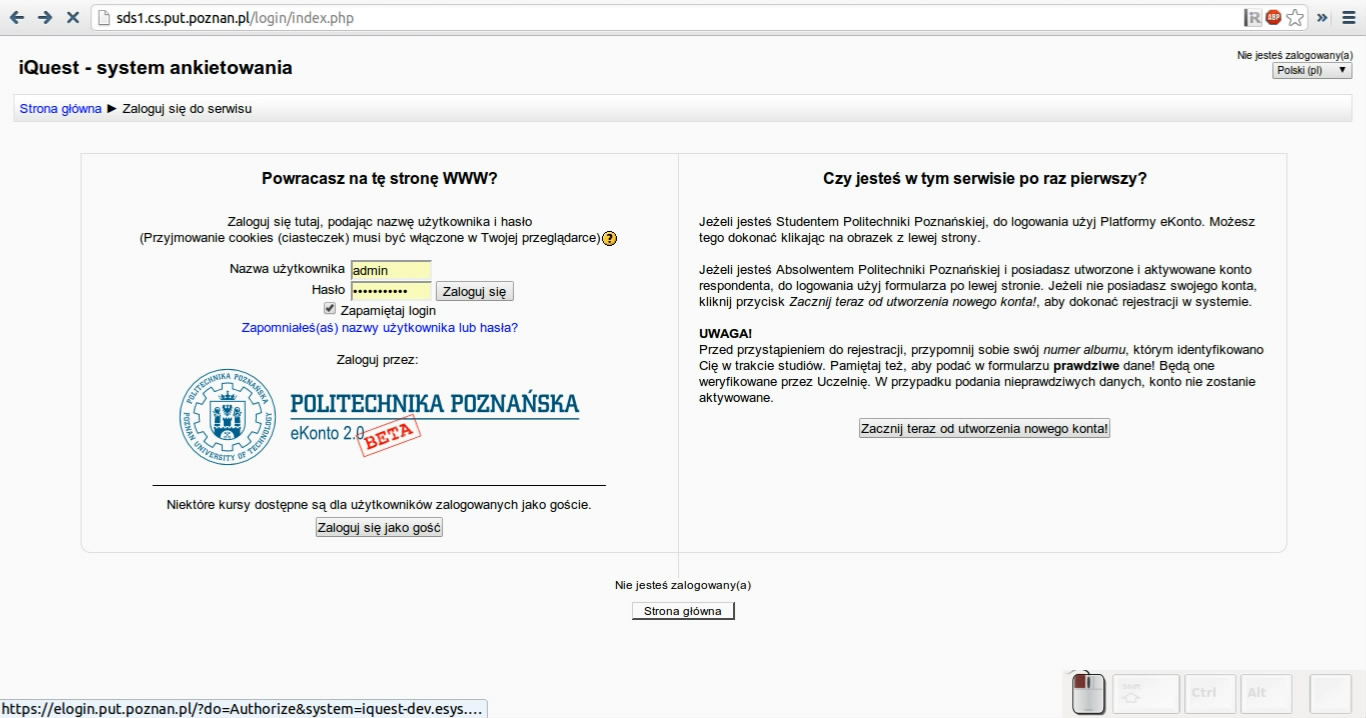
\includegraphics[width=0.9\textwidth]{figures/kb/W2-logowanie}
\caption{Logowanie do systemu \textit{iQuest} (wyk. Krzysztof Marian Borowiak)}\label{rys:Logowanie}
\end{figure}

\begin{figure}[H]
\centering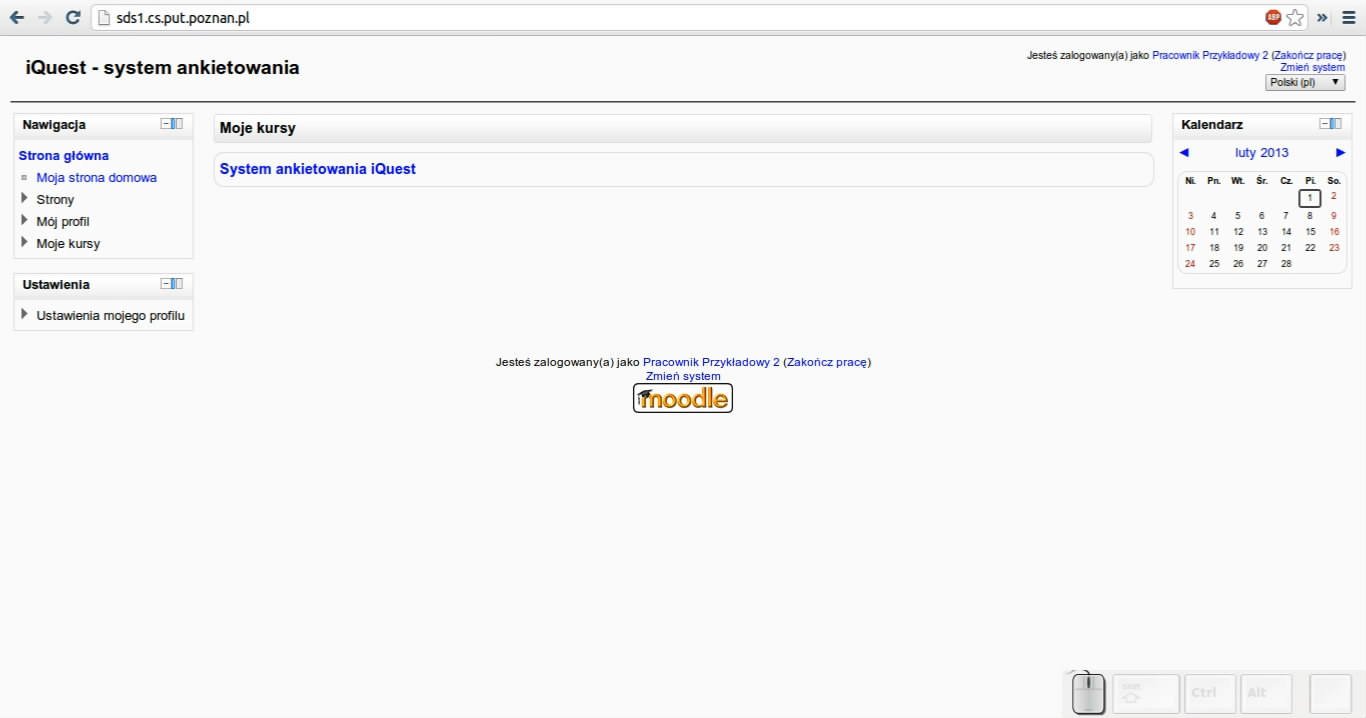
\includegraphics[width=0.9\textwidth]{figures/kb/W2-stronaglowna}
\caption{Strona główna systemu \textit{iQuest} -- widok ankietera (wyk. Krzysztof Marian Borowiak)}\label{rys:StronaGlowna}
\end{figure}

\begin{figure}[H]
\centering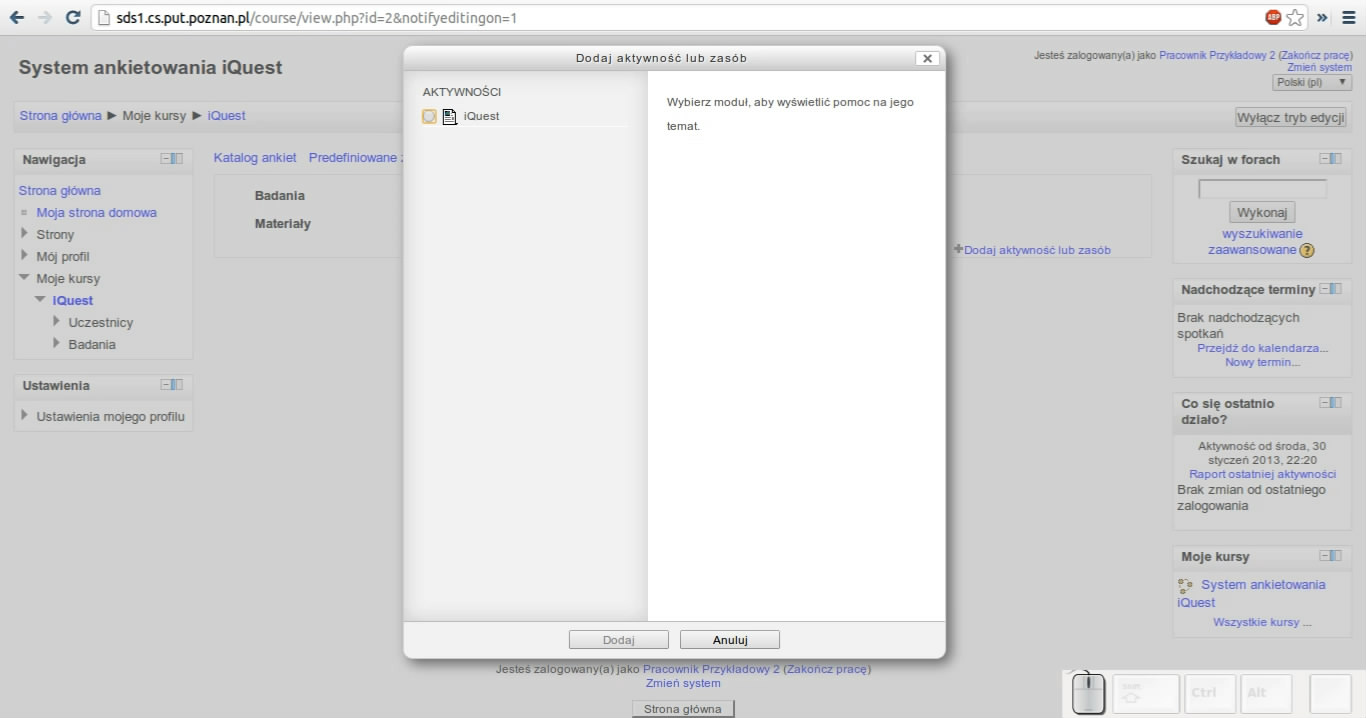
\includegraphics[width=0.9\textwidth]{figures/kb/W2-dodawaniebadania}
\caption{Dodawanie badania w systemie \textit{iQuest} (wyk. Krzysztof Marian Borowiak)}\label{rys:DodawanieBadania}
\end{figure}

\begin{figure}[H]
\centering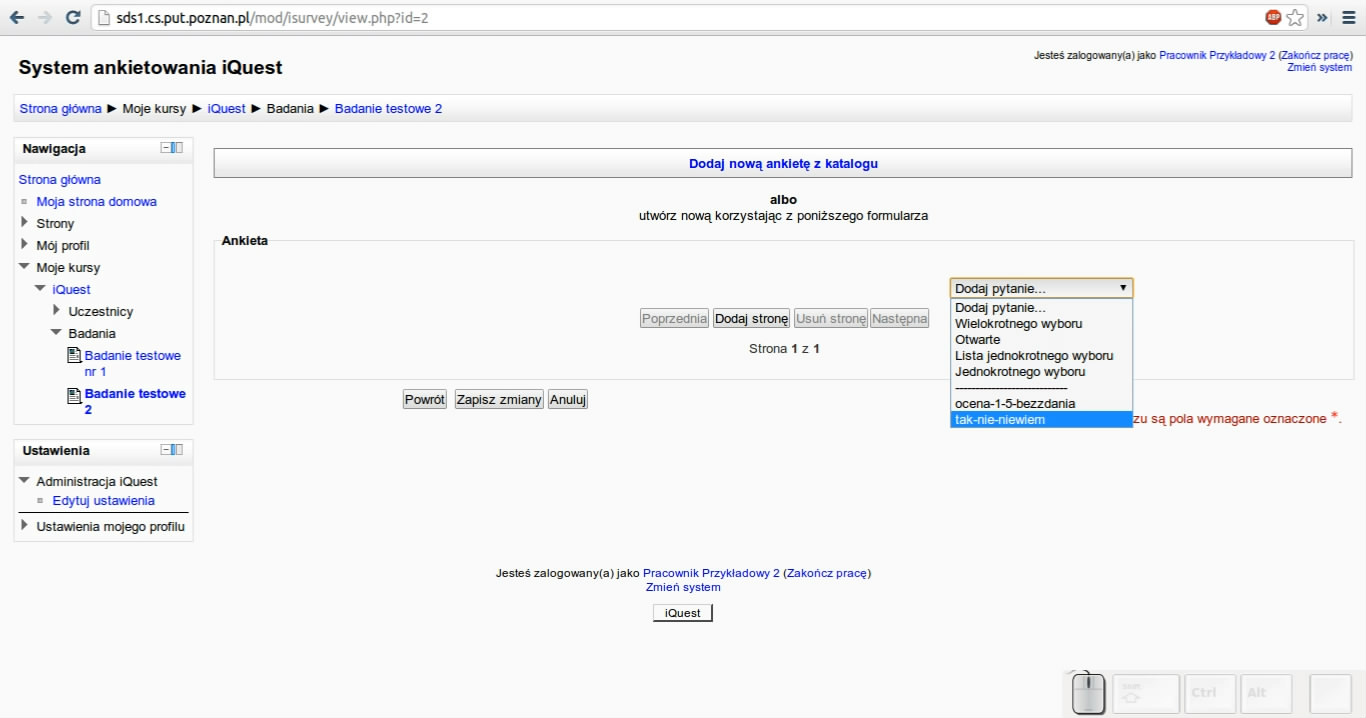
\includegraphics[width=0.9\textwidth]{figures/kb/W2-tworzenieankiety}
\caption{Tworzenie ankiety w systemie \textit{iQuest} -- wybór typu pytania (wyk. Krzysztof Marian Borowiak)}\label{rys:TworzenieAnkiety}
\end{figure}

\begin{figure}[H]
\centering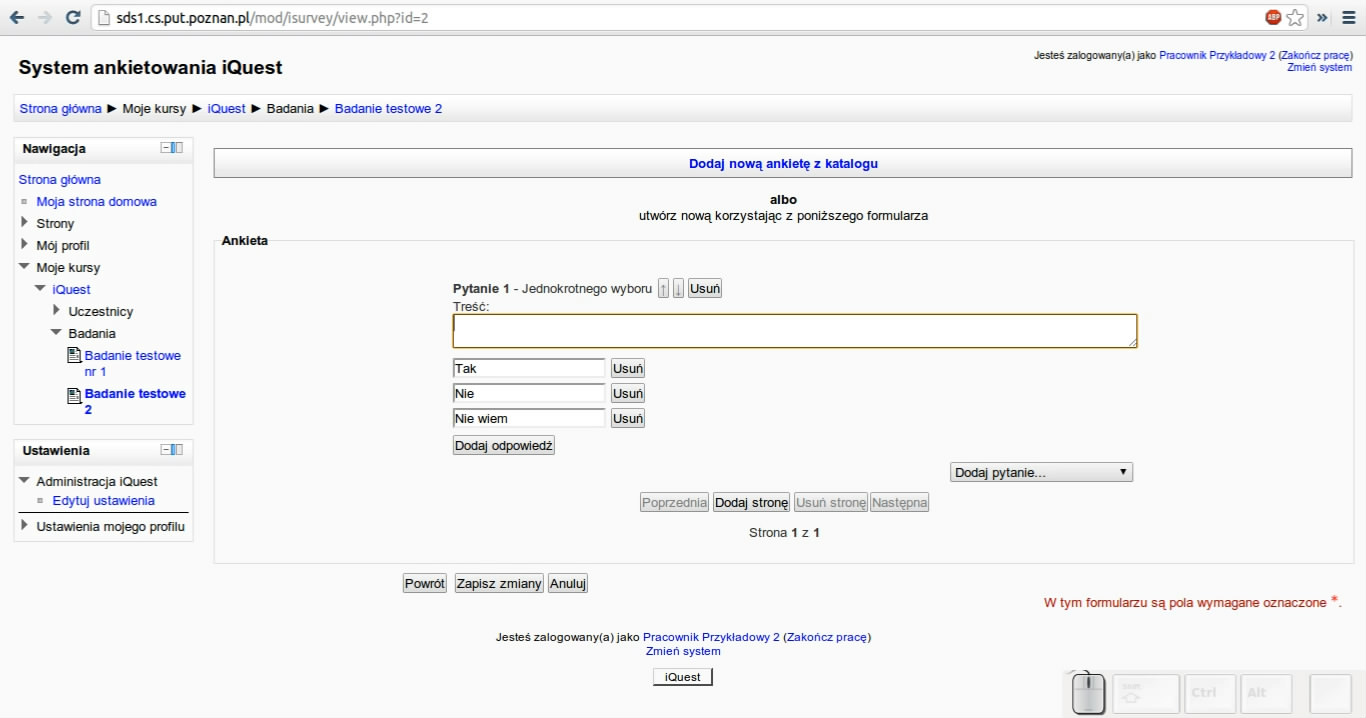
\includegraphics[width=0.9\textwidth]{figures/kb/W2-tworzenieankiety2}
\caption{Tworzenie ankiety w systemie \textit{iQuest} -- modyfikacja pytania (wyk. Krzysztof Marian Borowiak)}\label{rys:TworzenieAnkiety2}
\end{figure}

\begin{figure}[H]
\centering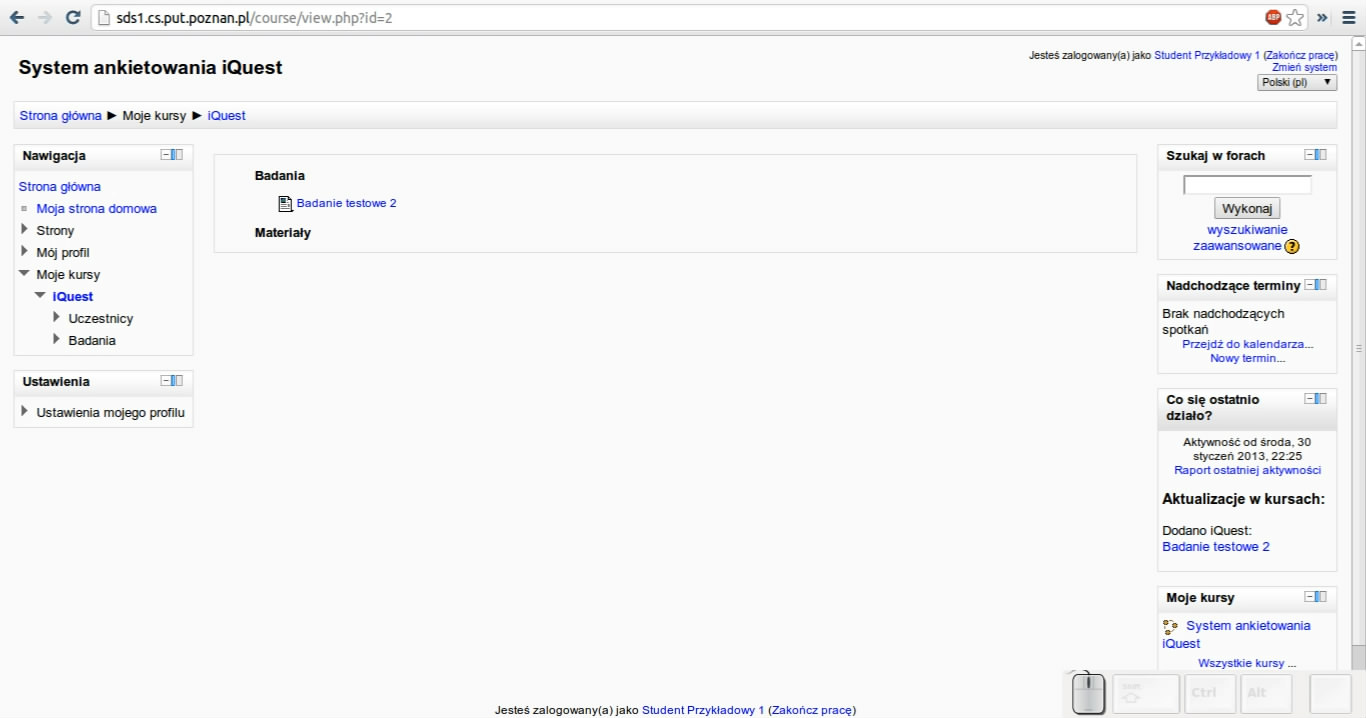
\includegraphics[width=0.9\textwidth]{figures/kb/W2-wyborbadania}
\caption{Lista badań dostępna dla respondenta (wyk. Krzysztof Marian Borowiak)}\label{rys:WyborBadania}
\end{figure}

\begin{figure}[H]
\centering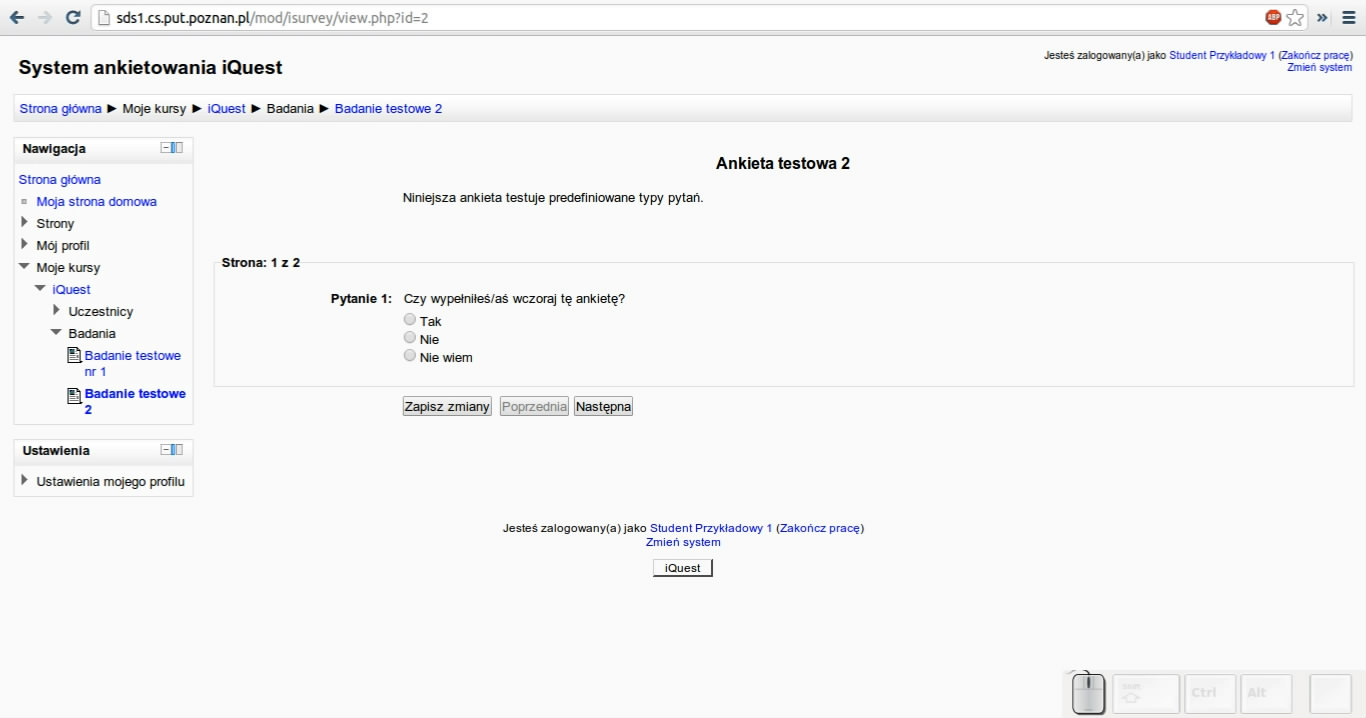
\includegraphics[width=0.9\textwidth]{figures/kb/W2-odpowiadanienanakiete}
\caption{Interfejs ankiety dla respondenta (wyk. Krzysztof Marian Borowiak)}\label{rys:OdpowiadanieNaAnkiete}
\end{figure}
\chapter{Schemat bazy danych}
\label{Chapterc1}

\begin{landscape}
\begin{figure}[th]
\centering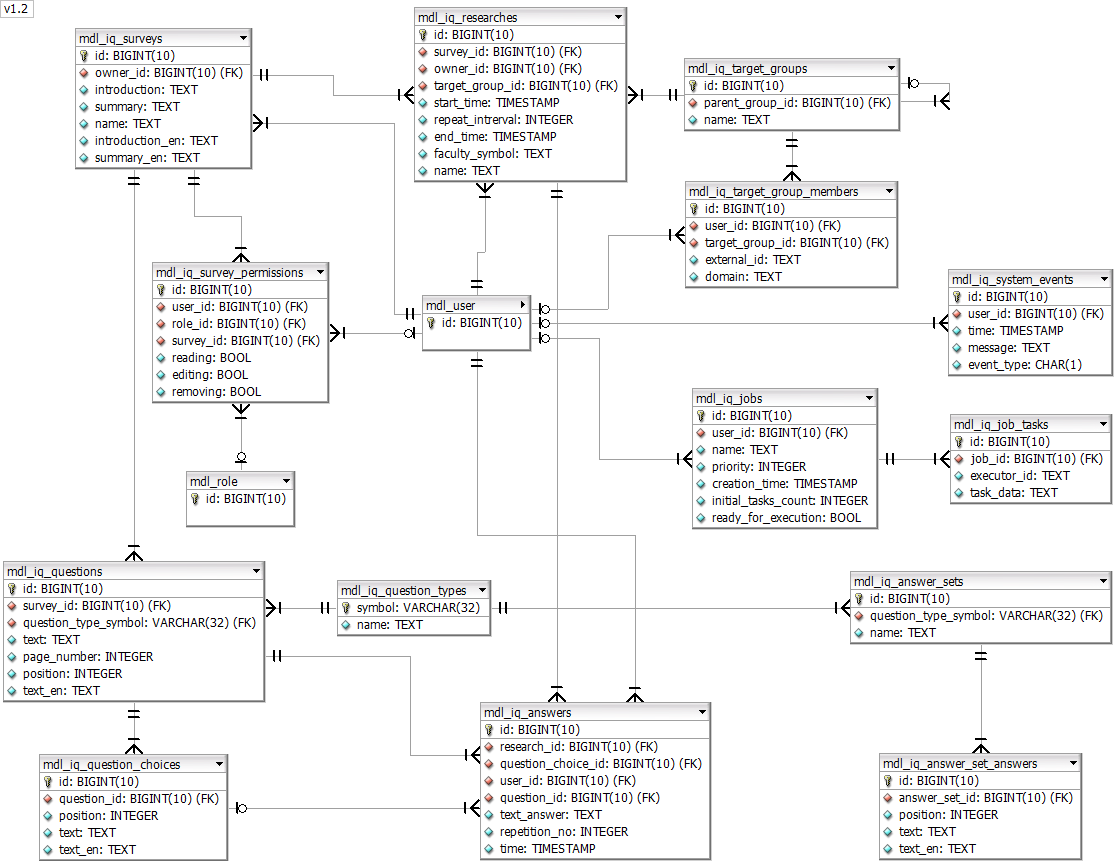
\includegraphics[height=\textheight, width=\textwidth]{figures/iQuest_Database}
\caption{Diagram Bazy Danych}\label{rys:iQuest_DataBase}
\end{figure}
\end{landscape}

% Bibliography (books, articles) starts here.
\bibliographystyle{plunsrt}{\raggedright\sloppy\small\bibliography{bibliography}}

% Colophon is a place where you should let others know about copyrights etc.
\ppcolophon

\end{document}
